
% !TeX spellcheck = en_GB
\documentclass{beamer}
\usepackage[utf8]{inputenc}
 \usetheme{antibes}
 \usepackage{movie15}
 \usepackage{graphicx}
 \usepackage{hyperref}
 \usepackage{tikz}
 \usetikzlibrary{shapes.geometric, arrows}
 \tikzstyle{startstop} = [rectangle, rounded corners, minimum width=3cm, minimum height=1cm,text centered, draw=blue, fill=blue!15]
 \tikzstyle{arrow} = [thick,->,>=stealth]
 \hypersetup{
 	colorlinks=true,
 	linkcolor=blue,
 	filecolor=magenta,      
 	urlcolor=cyan,
 }
 
 \urlstyle{same}
 \title[\textcolor{orange}{Karsten Moholt Digital}] %optional
 {Data science in predictive maintenance }
 
 \subtitle{An optimization probblem}
 
 \author[] % (optional, for multiple authors)
 {Yapi Donatien Achou}
 
% \institute[VFU] % (optional)
% {
% 	\inst{1}%
% 	Faculty of Physics\\
% 	Very Famous University
% 	\and
% 	\inst{2}%
% 	Faculty of Chemistry\\
% 	Very Famous University
% }
 
 %\date[VLC 2013] % (optional)
 %{Very Large Conference, April 2013}
 
 \logo{
\includegraphics[height=1.5cm]{km-logo.png}}
 
 
\begin{document}
 
\frame{\titlepage}
 
 
 %%%%%%%%%%%%%%%%%%%%%%%%%%%%%%%%%%%%%%%%%%%%%%%%%%%%%%%%%%%
 
 
 
 %%%%%%%%%%%%%%%%%%%%%%%%%%%%%%%%%%%%%%%%%%%%%%%%%%%%%%%%%%%%
 
\begin{frame}
\frametitle{Data science is a multidisciplinary field}
\begin{figure}[H]
	\centering
	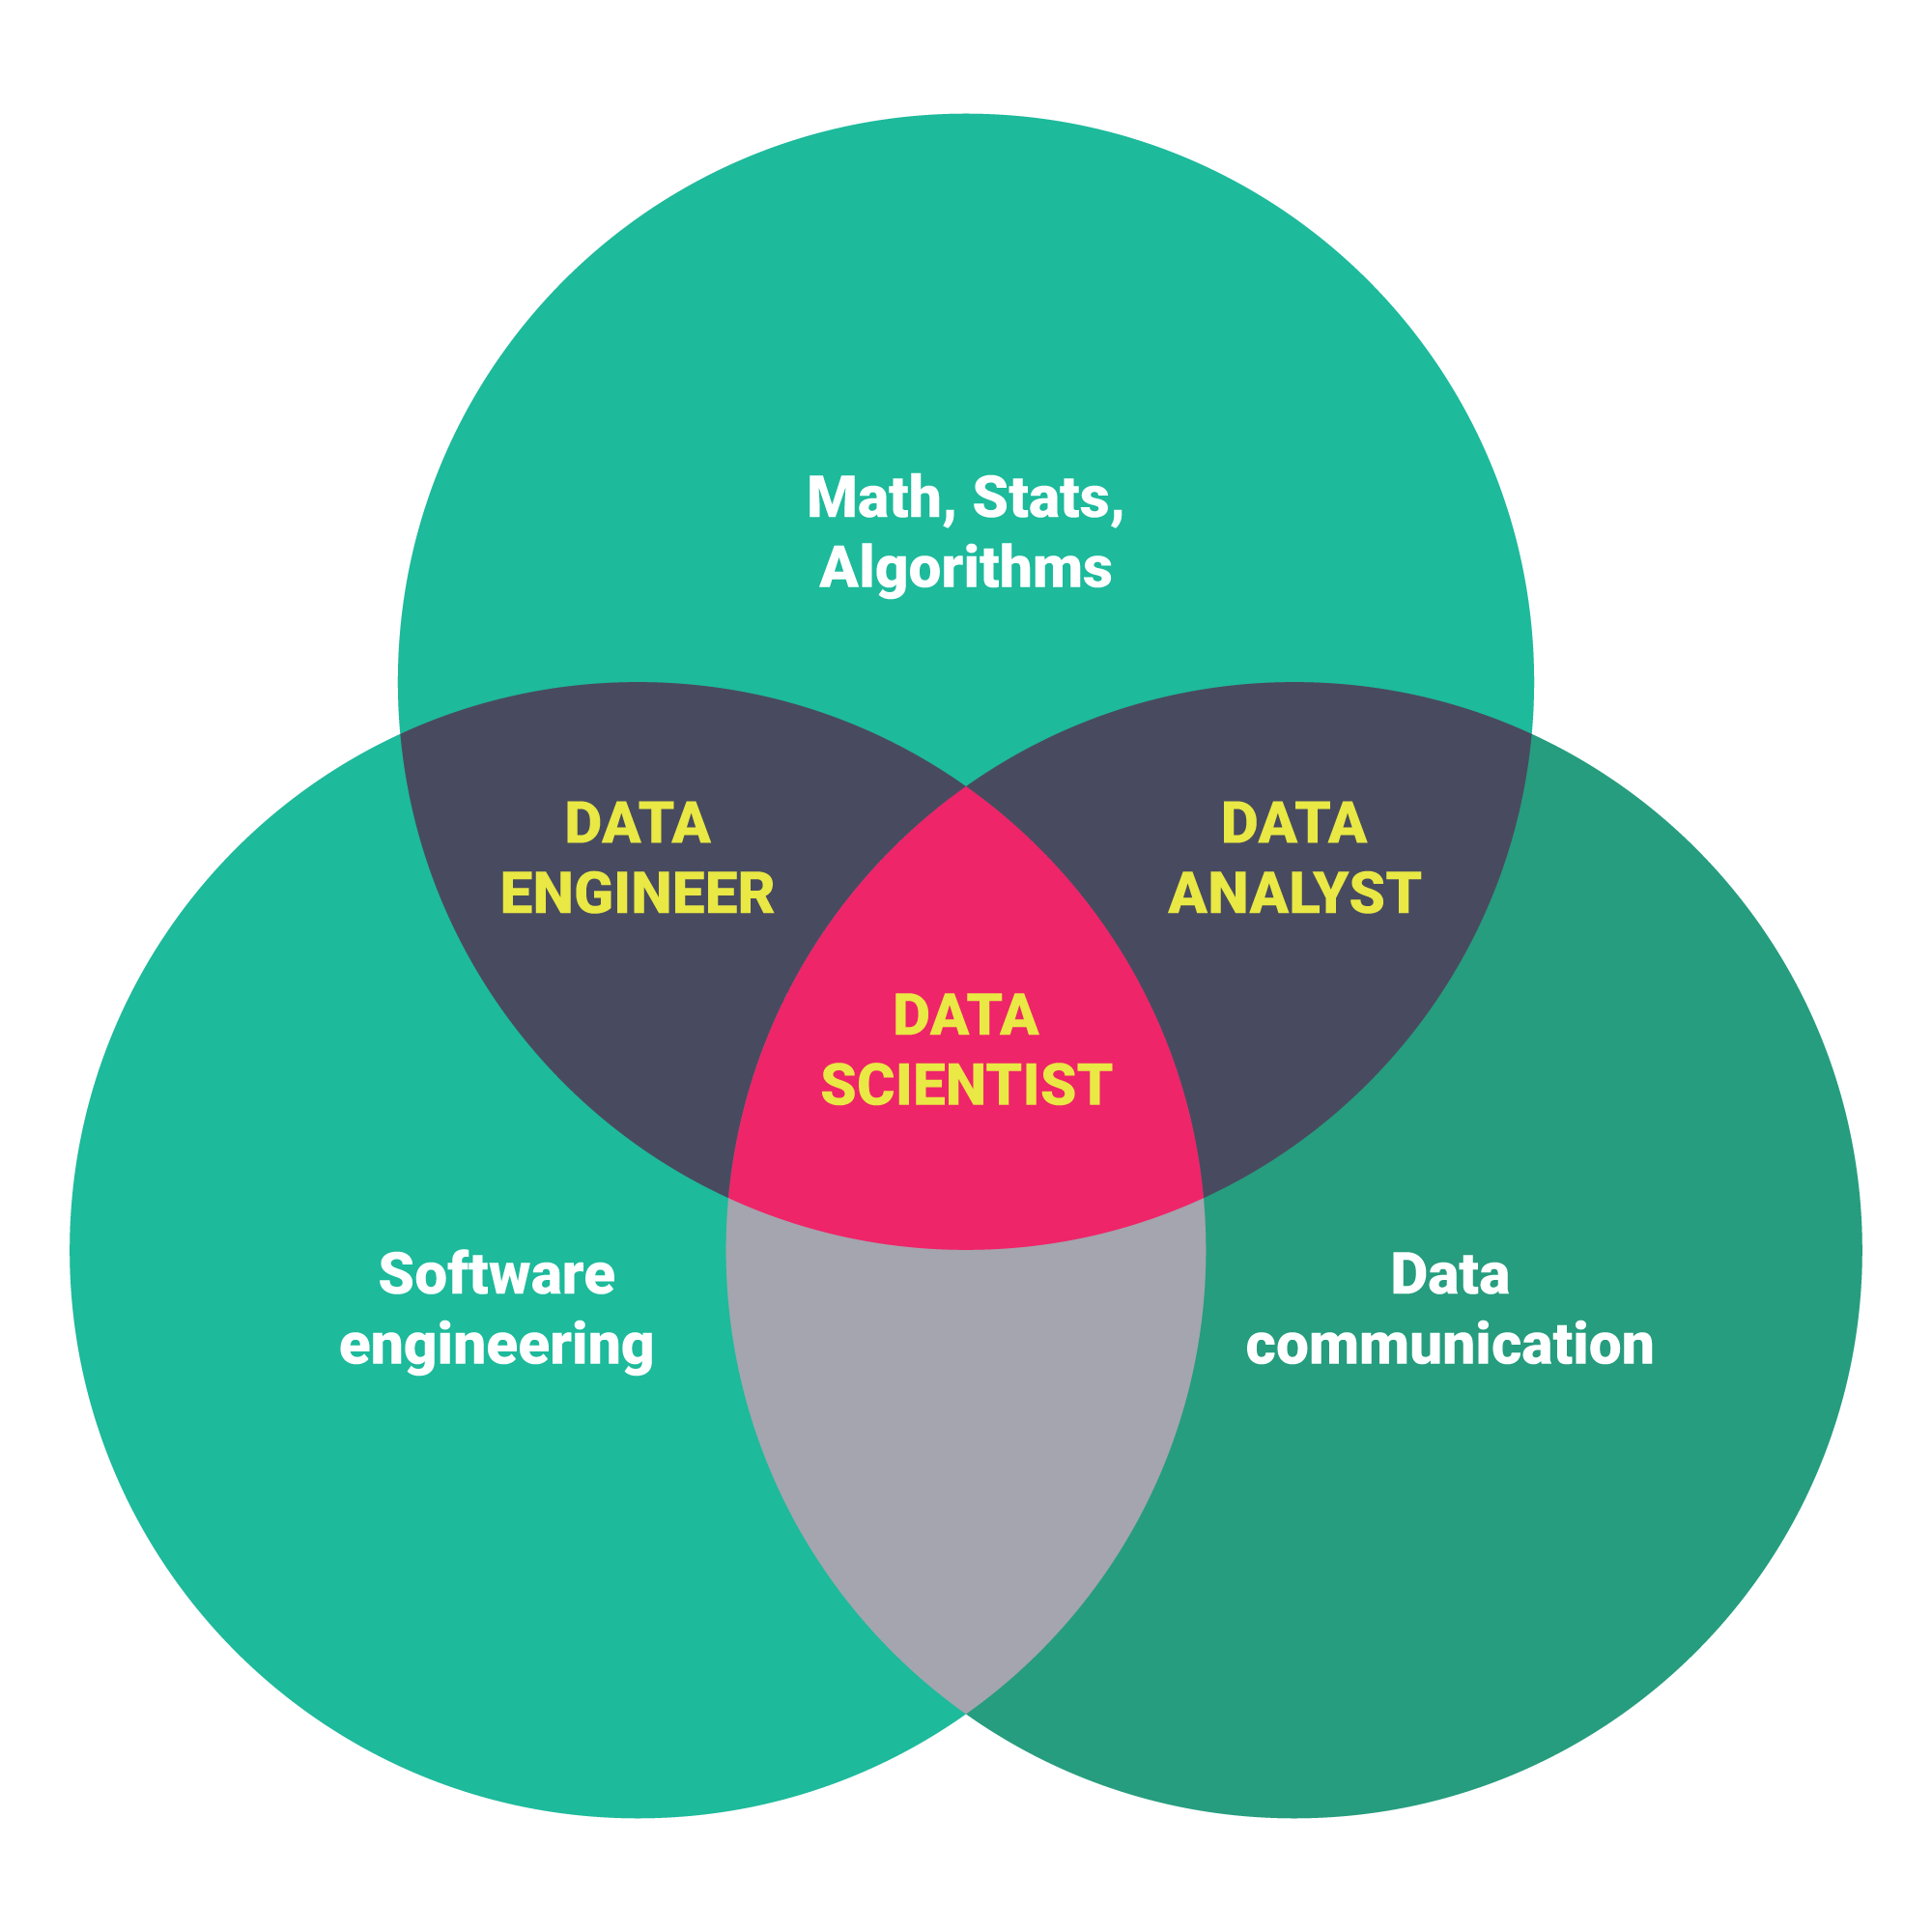
\includegraphics[width=0.4\linewidth]{datascience2}
	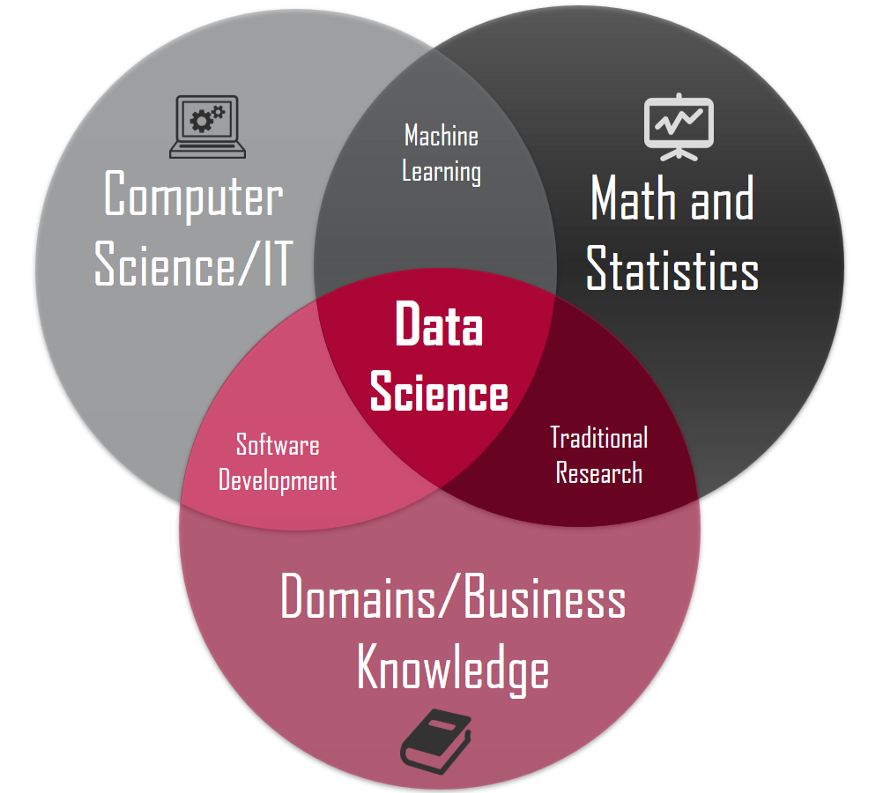
\includegraphics[width=0.4\linewidth]{datascience}
	%\caption{}
	%\label{fig:datascience}
\end{figure}
\end{frame}
%%%%%%%%%%%%%%%%%%%%%%%%%%%%%%%%%%%%%%%%%%%%%%%%%%%%%%
\begin{frame}
	\frametitle{Data science optimizes processes}
	\begin{figure}[H]
		\centering
		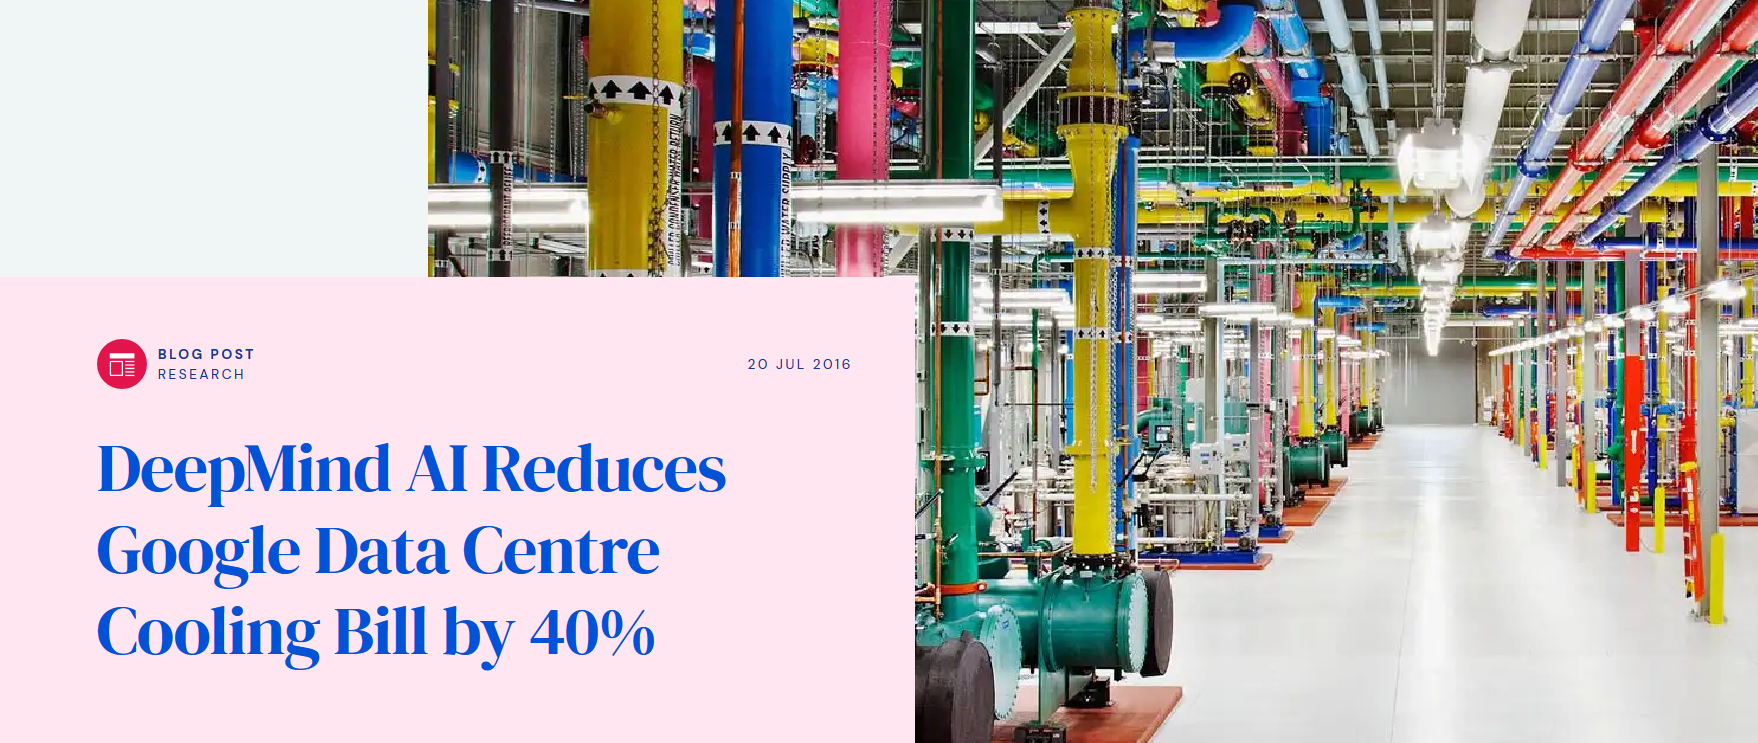
\includegraphics[width=1\linewidth]{google-data-center}
		%\caption{}
		%\label{fig:datascience}
	\end{figure}
\end{frame}


%%%%%%%%%%%%%%%%%%%%%%%%%%%%%%%%%%%%%%%%%%%%%%%%%%%%%%%%
\begin{frame}
	\frametitle{Data science methodology: \textcolor{orange}{A data driven modelling}}
\begin{figure}[H]
	\begin{center}
		\begin{tikzpicture}
\node (process) [startstop] {\textcolor{blue}{Process}};
\node (data) [startstop, below of=process, yshift=-1cm] {\textcolor{blue}{Data}};
\node (model) [startstop, below of=data, yshift=-1cm] {\textcolor{blue}{Model}};

%%% drawing %%%%%%%%%%%%%%%%%%%%%%%
\draw [arrow] (process) -- (data);
\draw [arrow] (data) -- (model);
		\end{tikzpicture}
	\end{center}

\end{figure}
\end{frame}
%%%%%%%%%%%%%%%%%%%%%%%%%%%%%%%%%%%%%%%%%%%%%%%%%%%%%%%%
\begin{frame}
	\frametitle{Data science methodology: \textcolor{orange}{Process conceptual model}}
\begin{figure}[H]
	\hspace*{-2cm} 
	%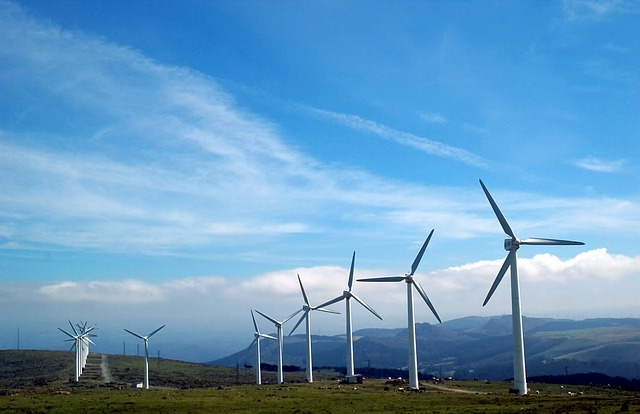
\includegraphics[width=0.2\linewidth]{windmil}
	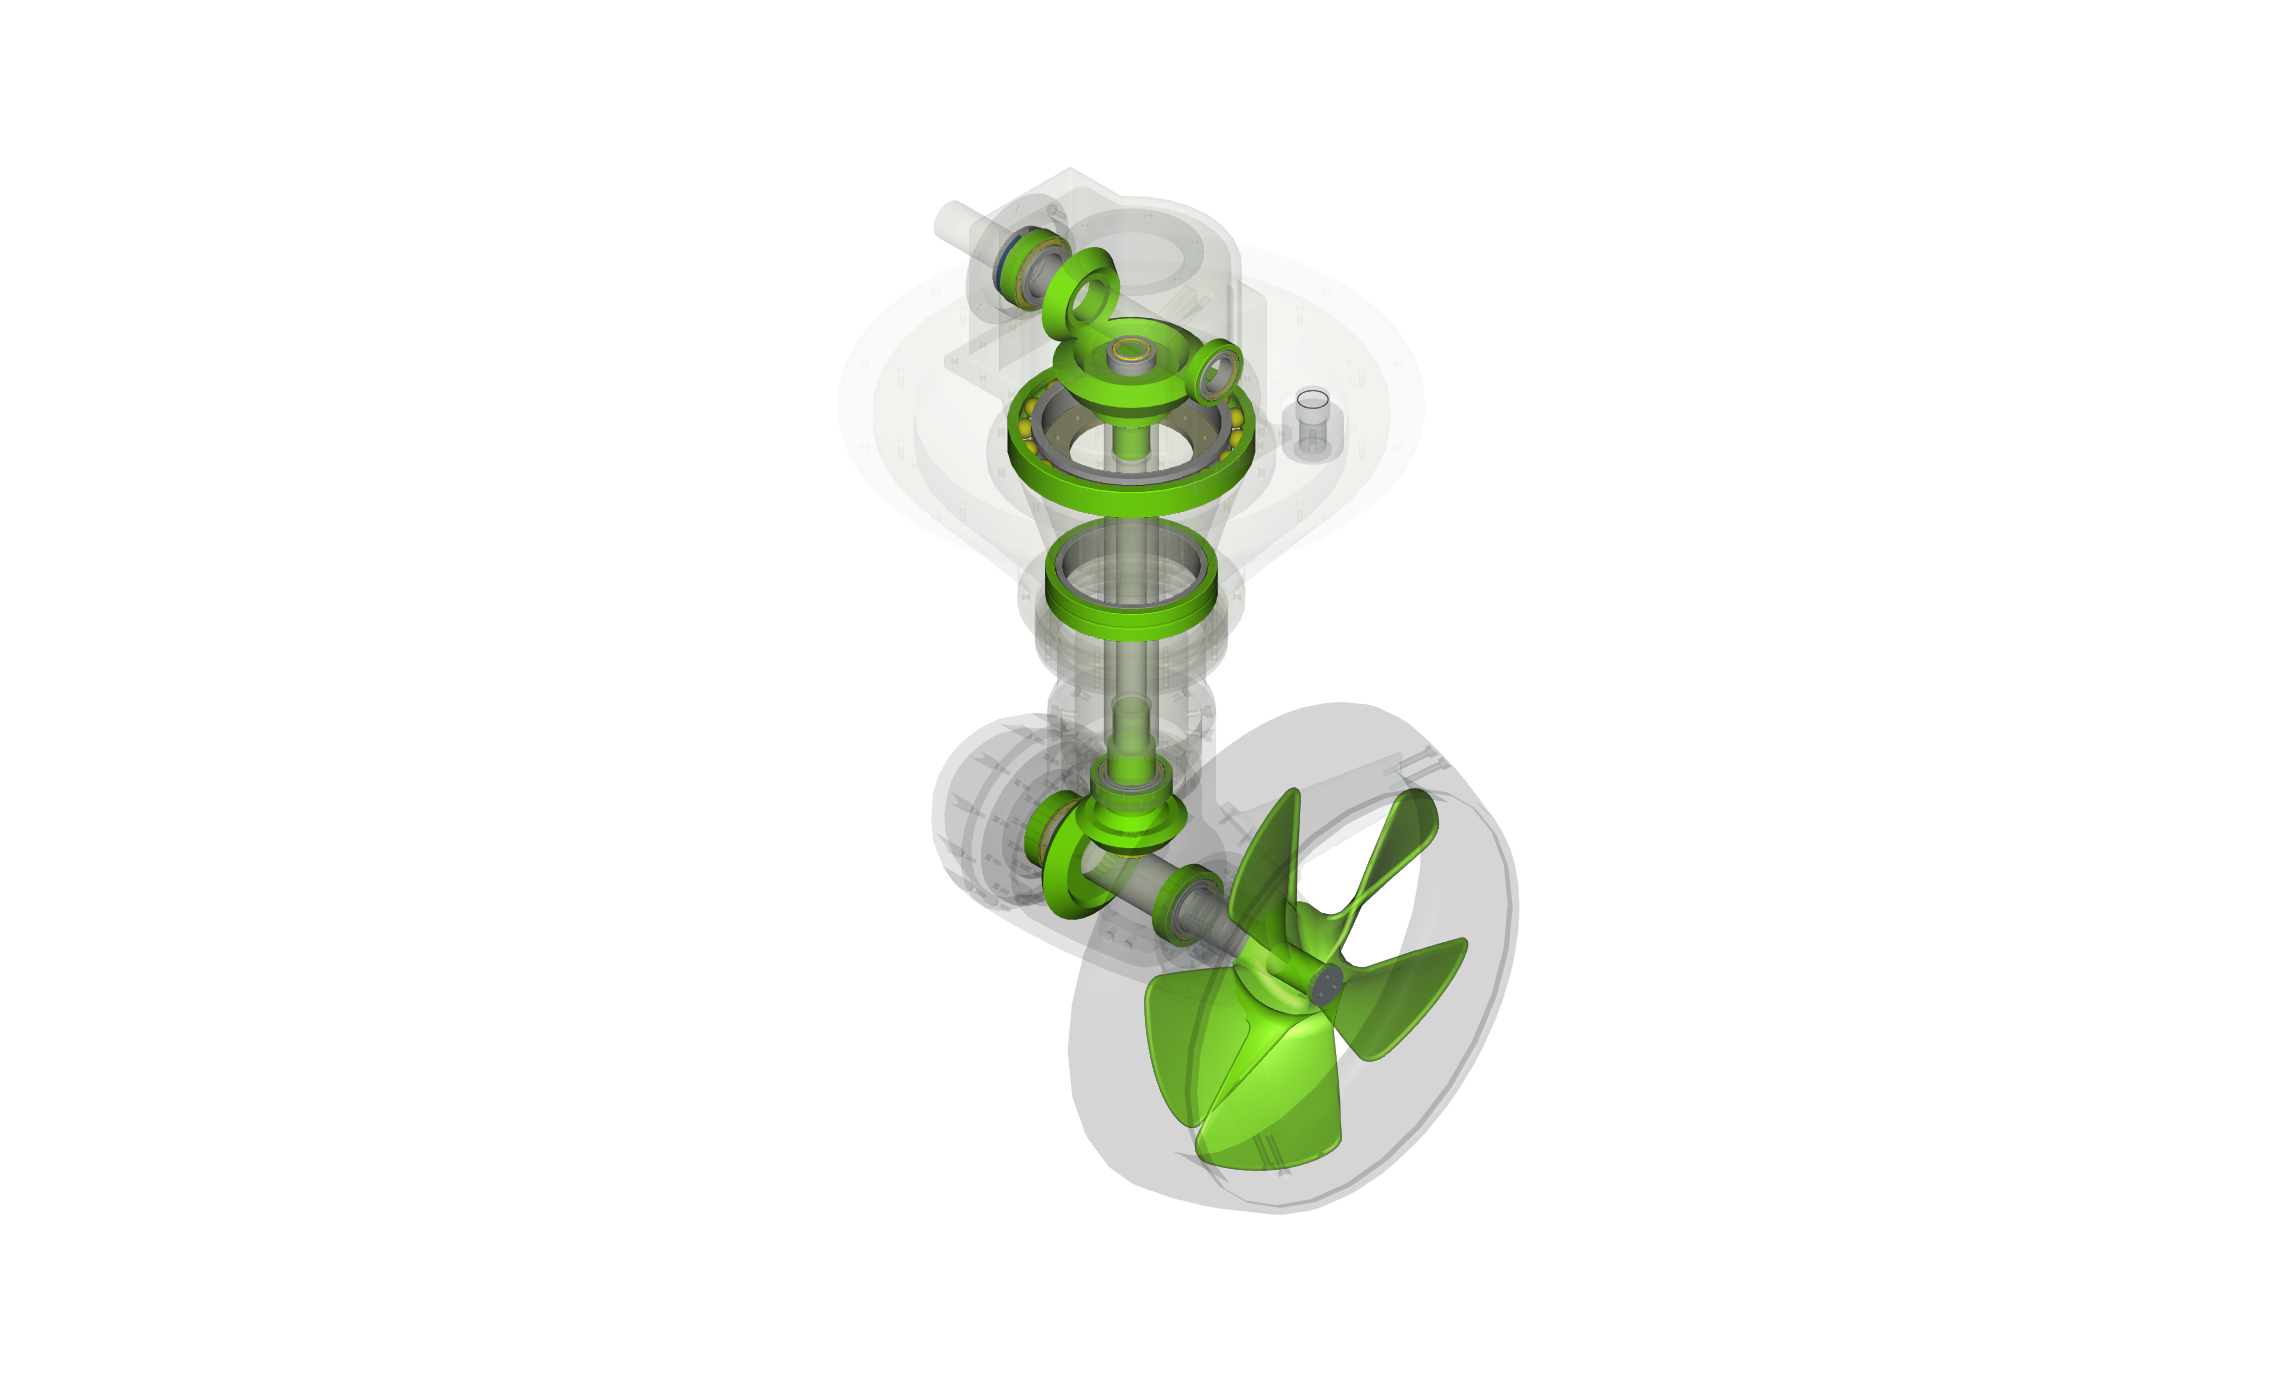
\includegraphics[width=0.8\linewidth]{thruster}
	%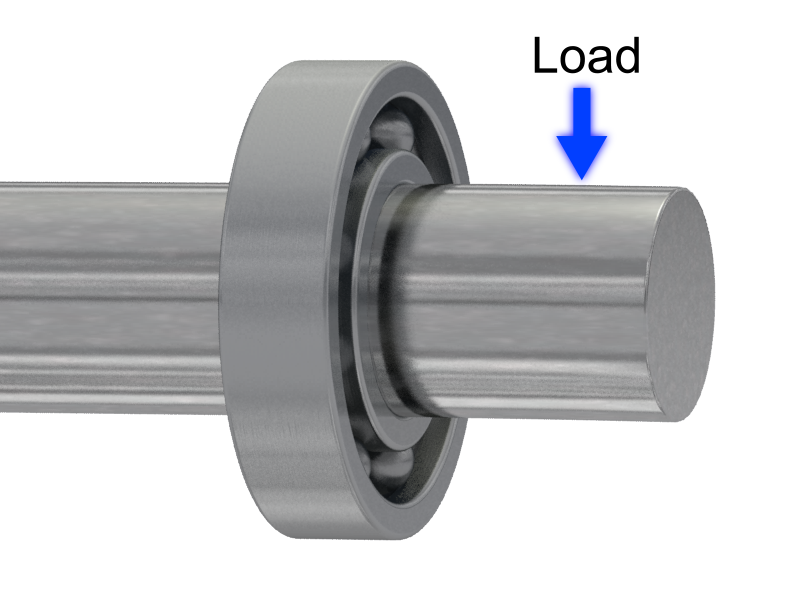
\includegraphics[width=0.2\linewidth]{bearing}
	%
\includegraphics[width=0.1\linewidth]{arrow}
	%
\includegraphics[width=0.15\linewidth]{conceptual}
\end{figure}
\end{frame}

\begin{frame}
	\frametitle{Data science methodology: \textcolor{orange}{Data quality and understanding}}
\begin{figure}[H]
	\centering
	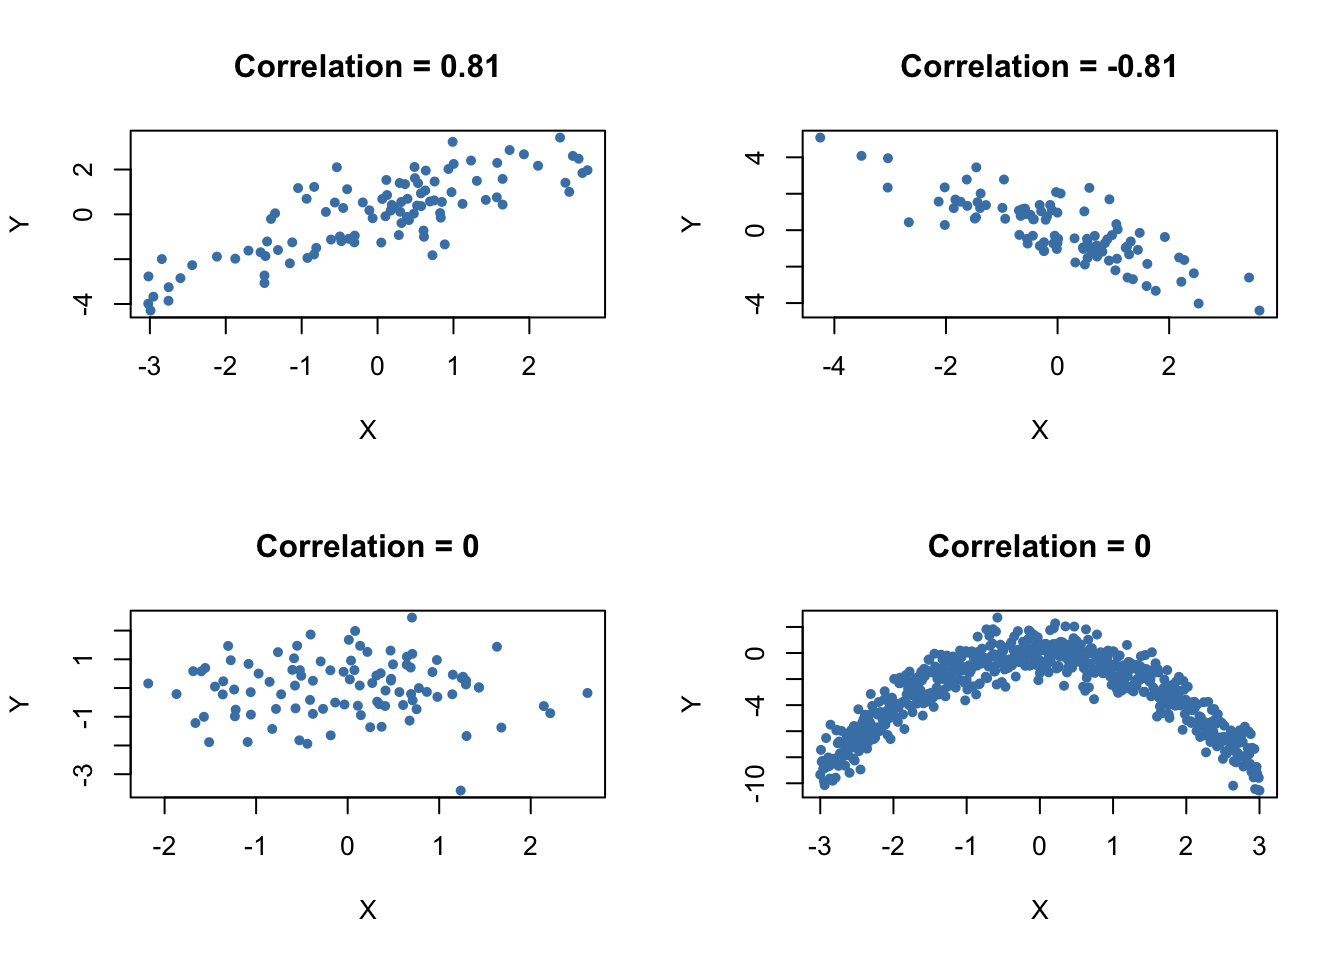
\includegraphics[width=0.4\linewidth]{data1}
	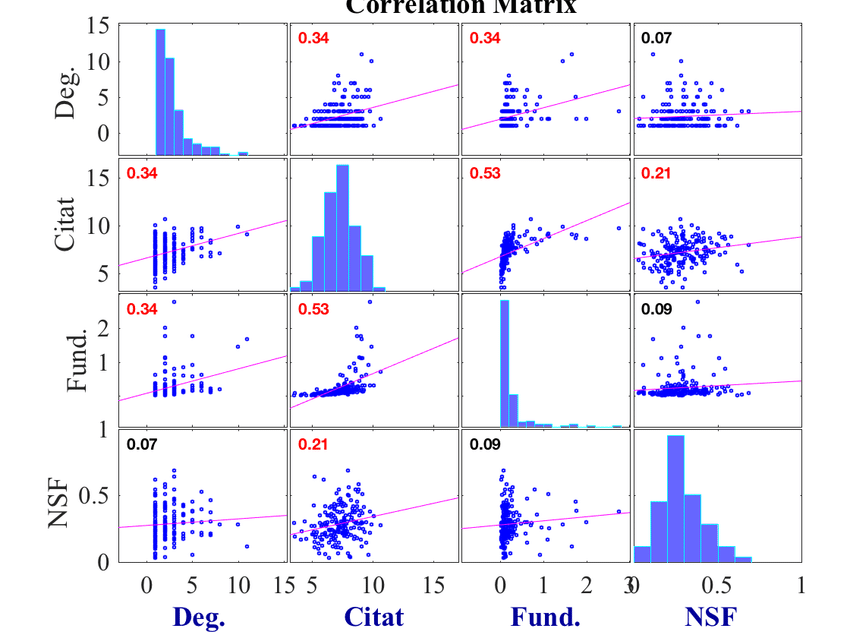
\includegraphics[width=0.4\linewidth]{data2}
	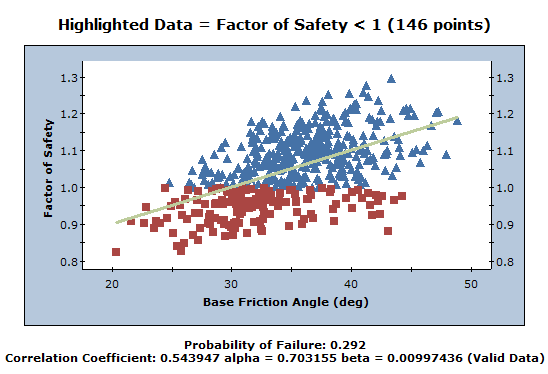
\includegraphics[width=0.4\linewidth]{data3}
\end{figure}
\end{frame}
%%%%%%%%%%%%%%%%%%%%%%%%%%%%%%%%%%%%%%%%%%%%%%%%%%%%%%%%
\begin{frame}
	\frametitle{Data science methodology: \textcolor{orange}{Model}}
\begin{figure}[H]
	\centering
	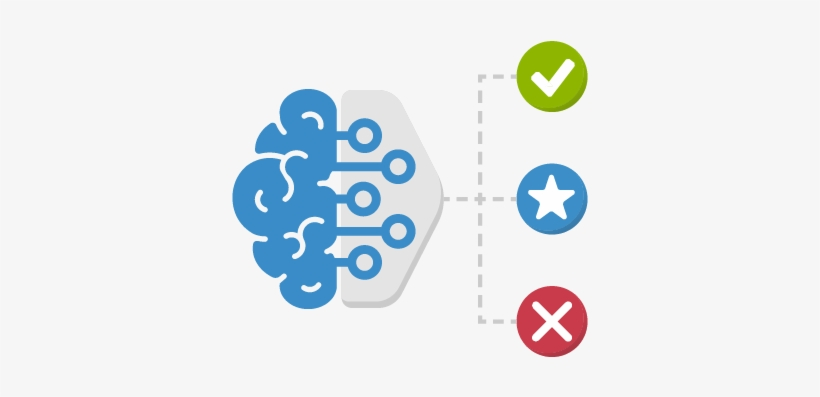
\includegraphics[width=0.9\linewidth]{model1}
\end{figure}
\begin{enumerate}
	\item Defect diagnosis
	\item Asset remaining useful life estimation
\end{enumerate}
\end{frame}
%%%%%%%%%%%%%%%%%%%%%%%%%%%%%%%%%%%%%%%%%%%%%%%%%%
\begin{frame}
	\frametitle{Data science in methodology: \textcolor{orange}{Analytics at scale}}
	\begin{figure}[H]
		\centering
		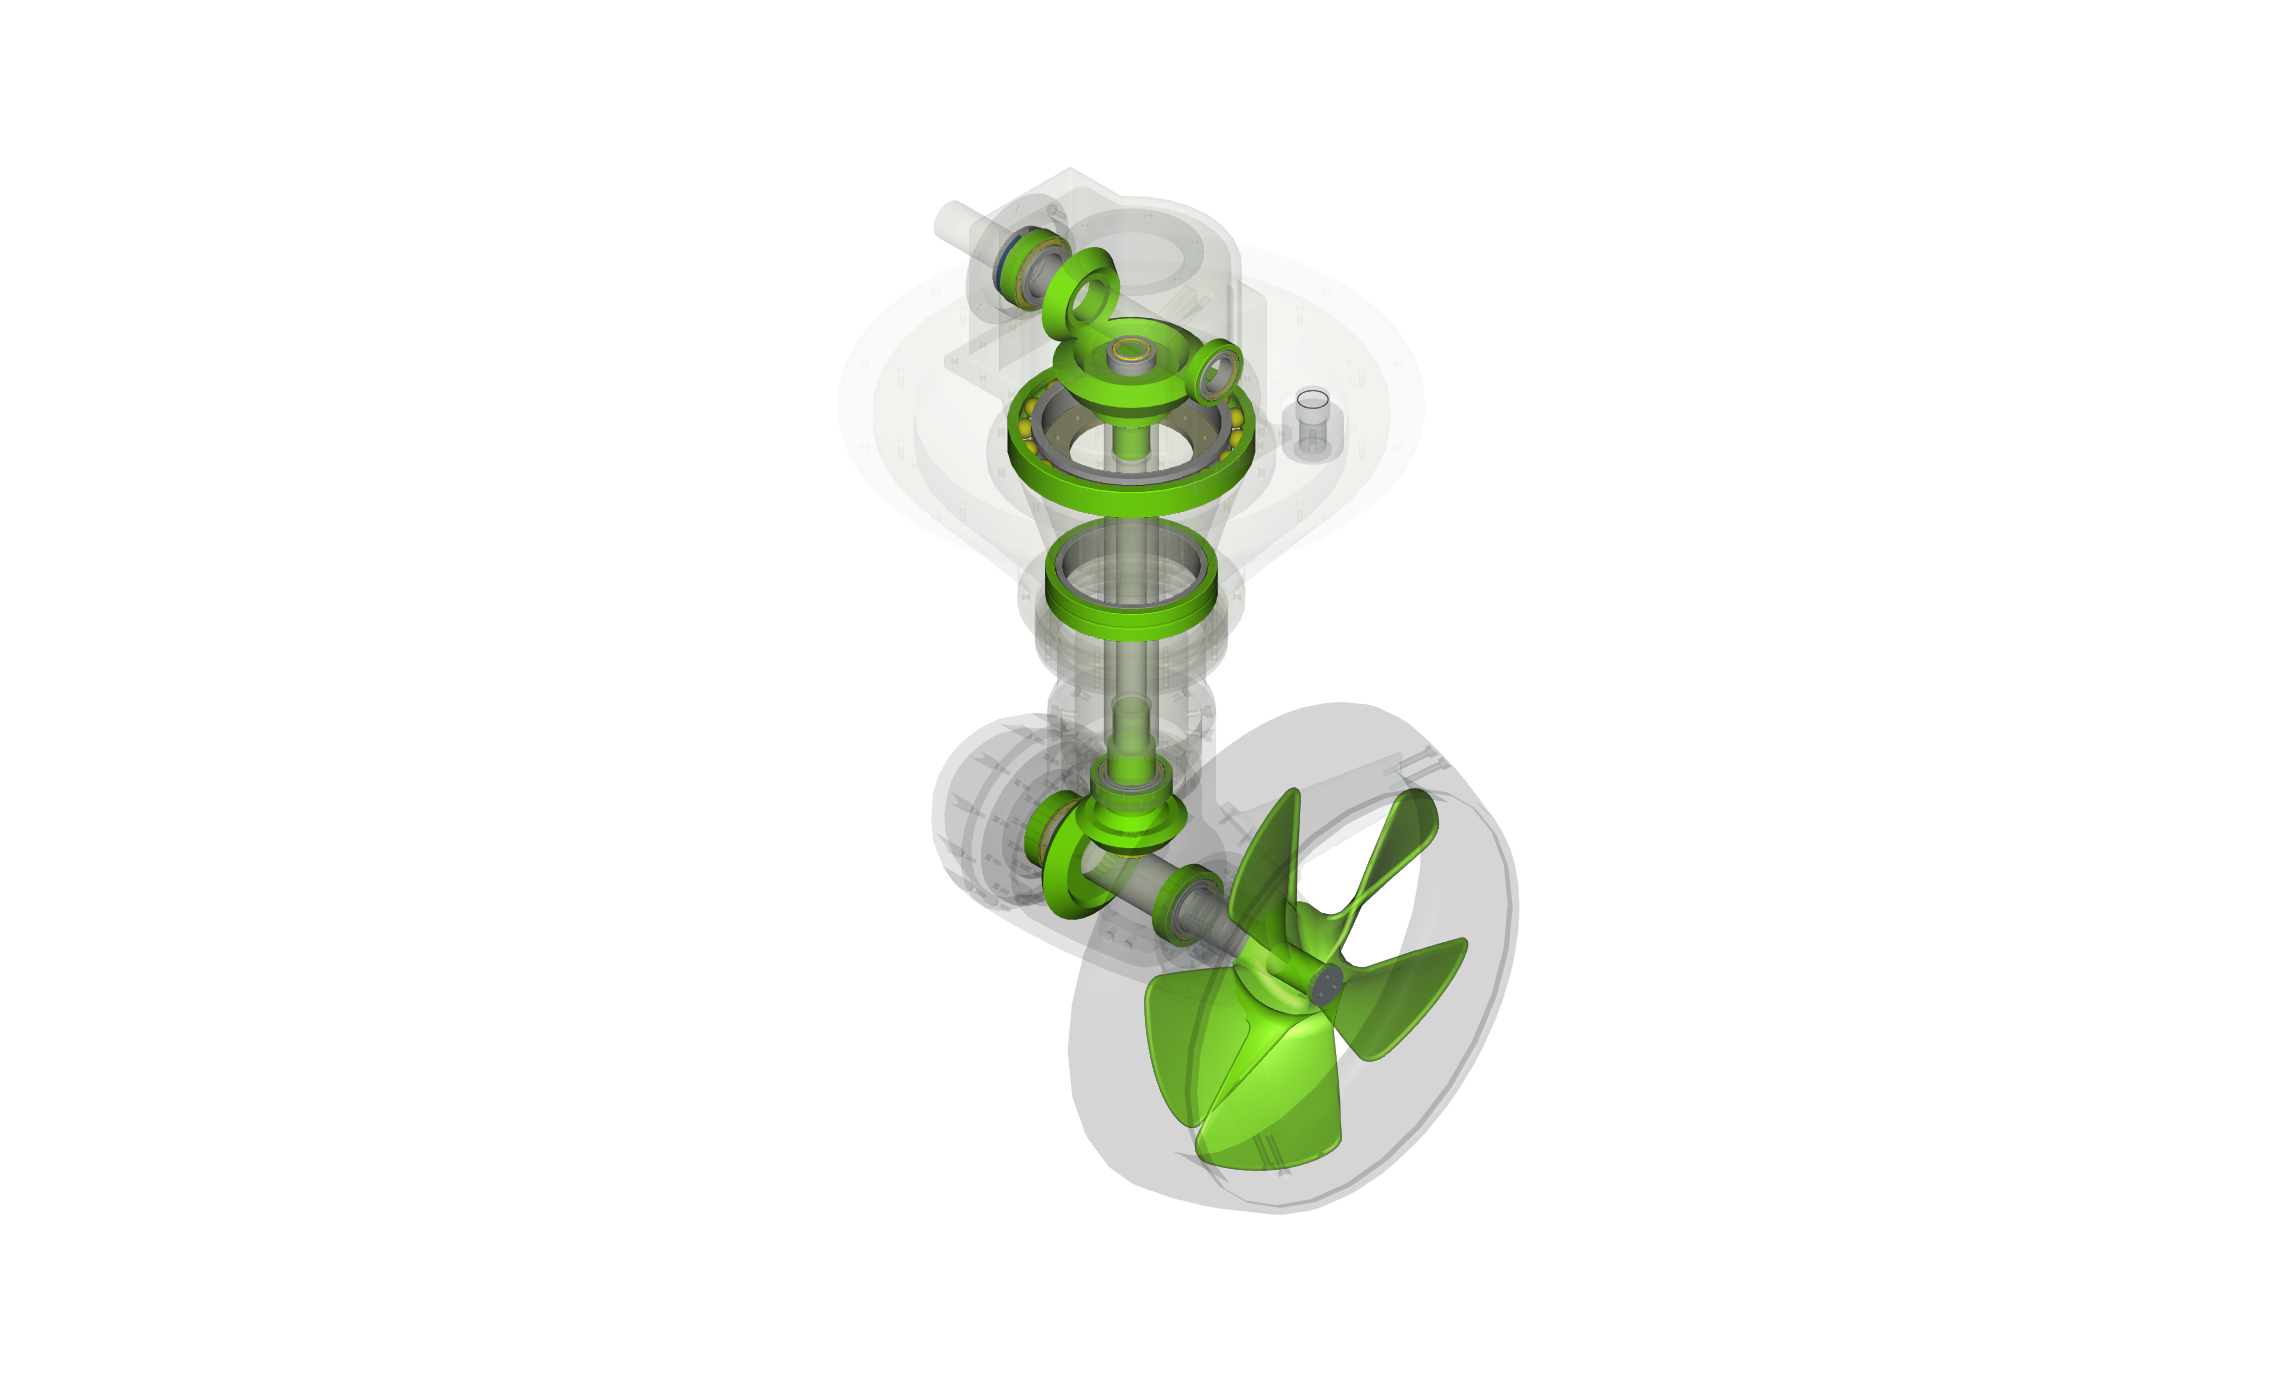
\includegraphics[width=0.3\linewidth]{thruster}
		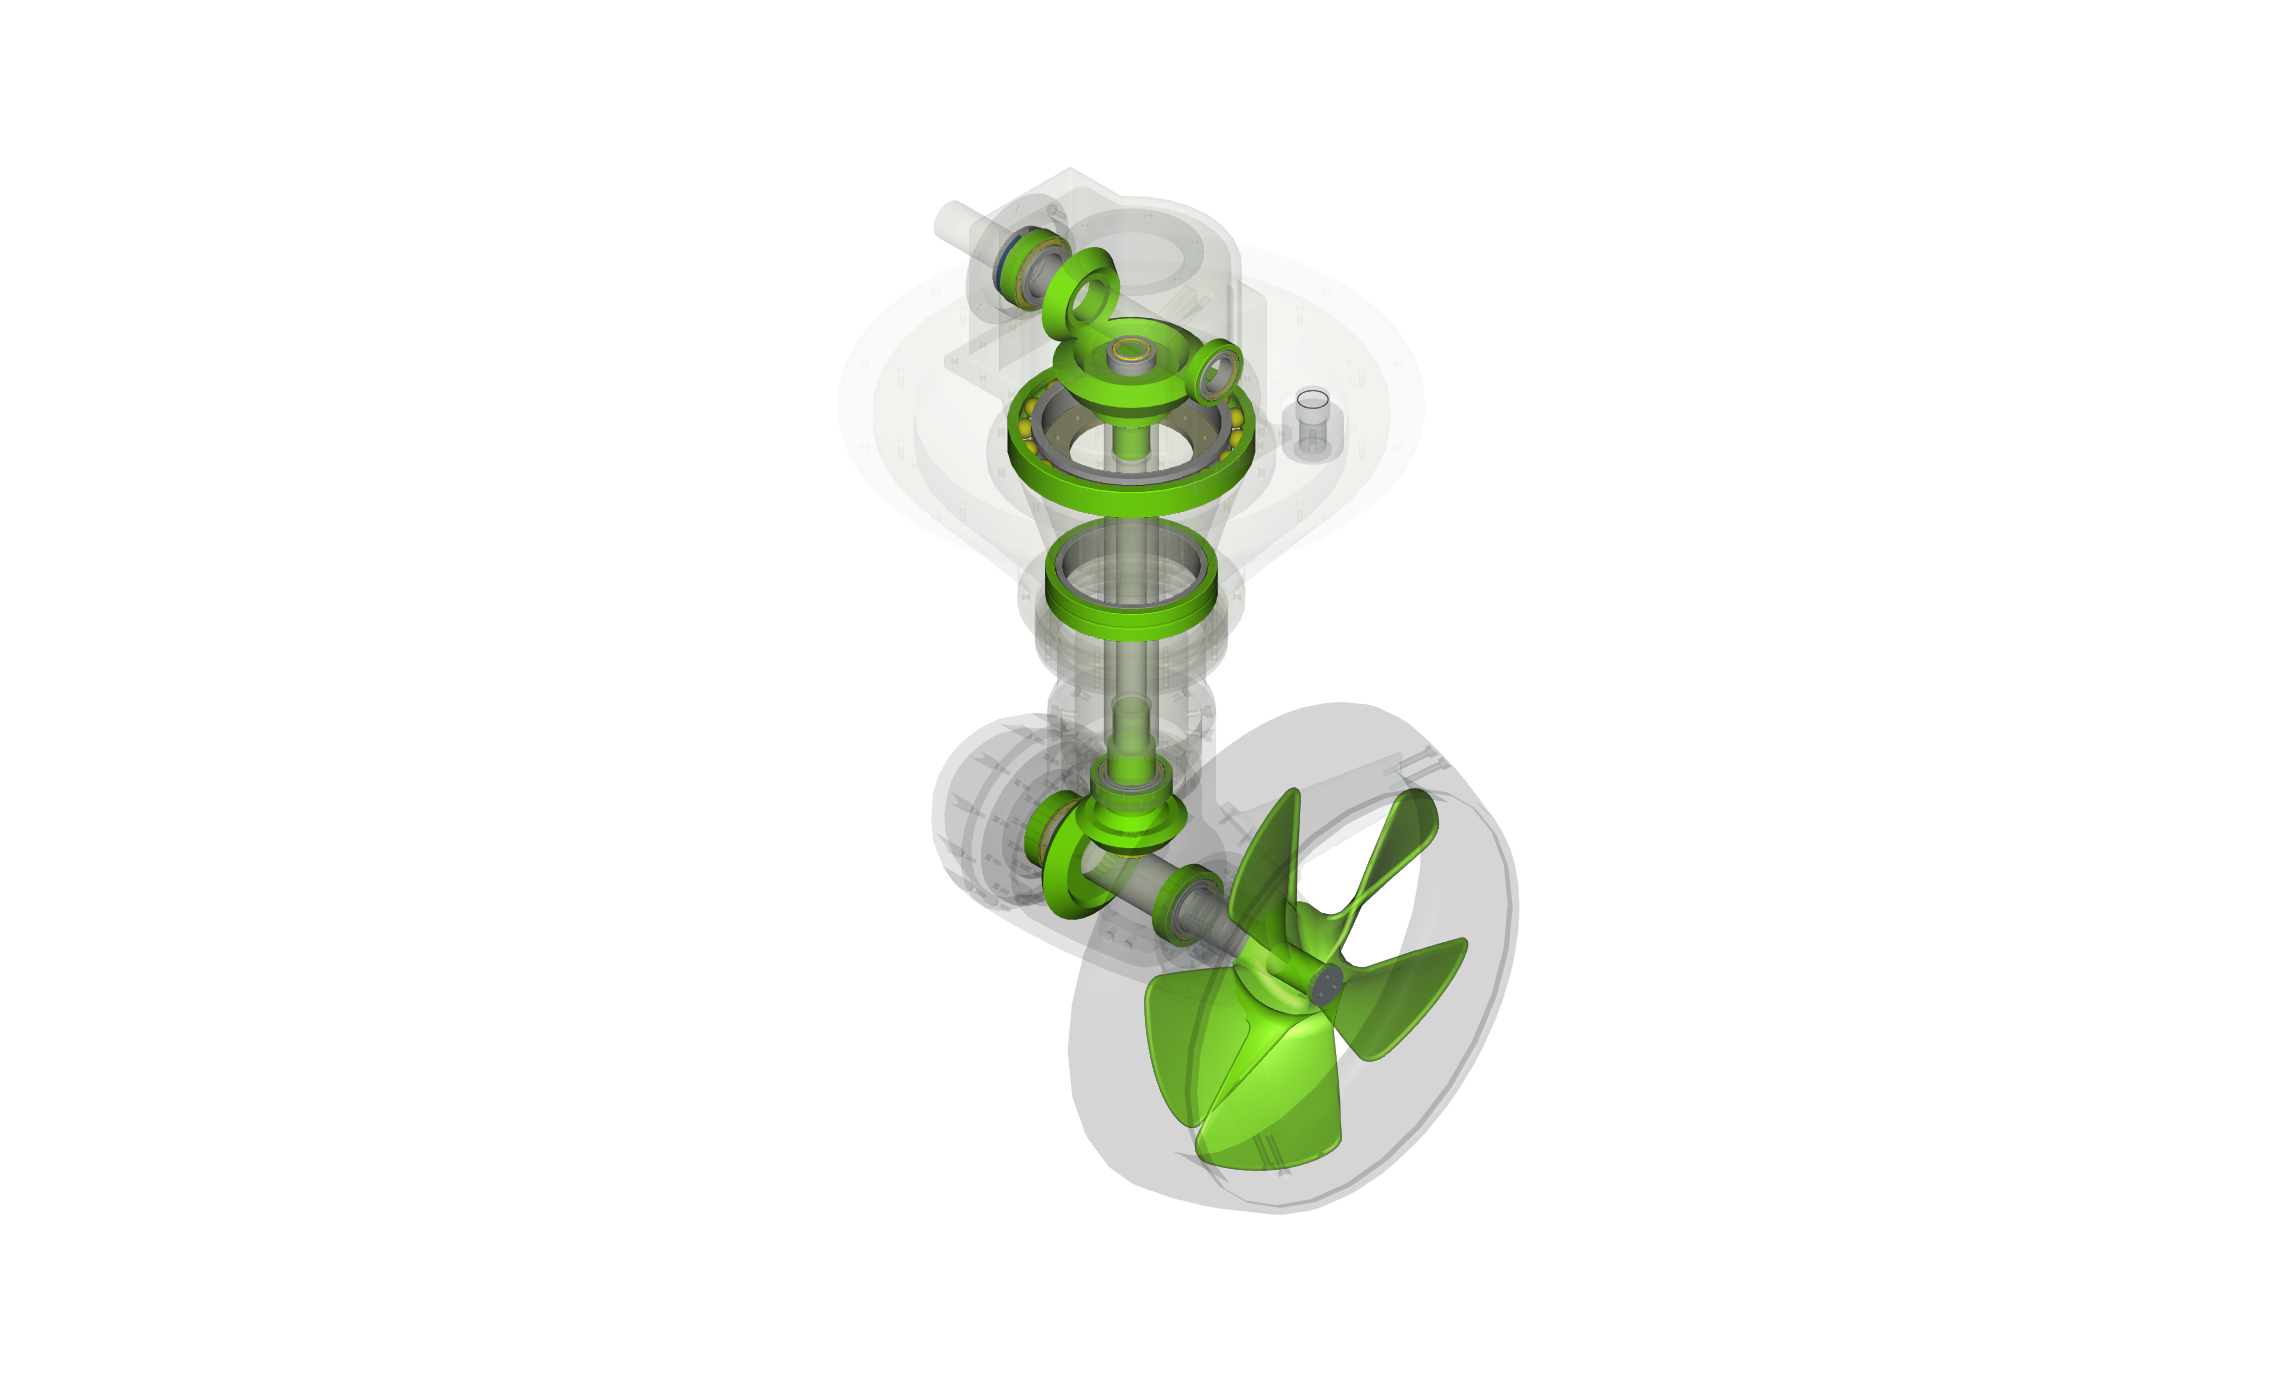
\includegraphics[width=0.3\linewidth]{thruster}
		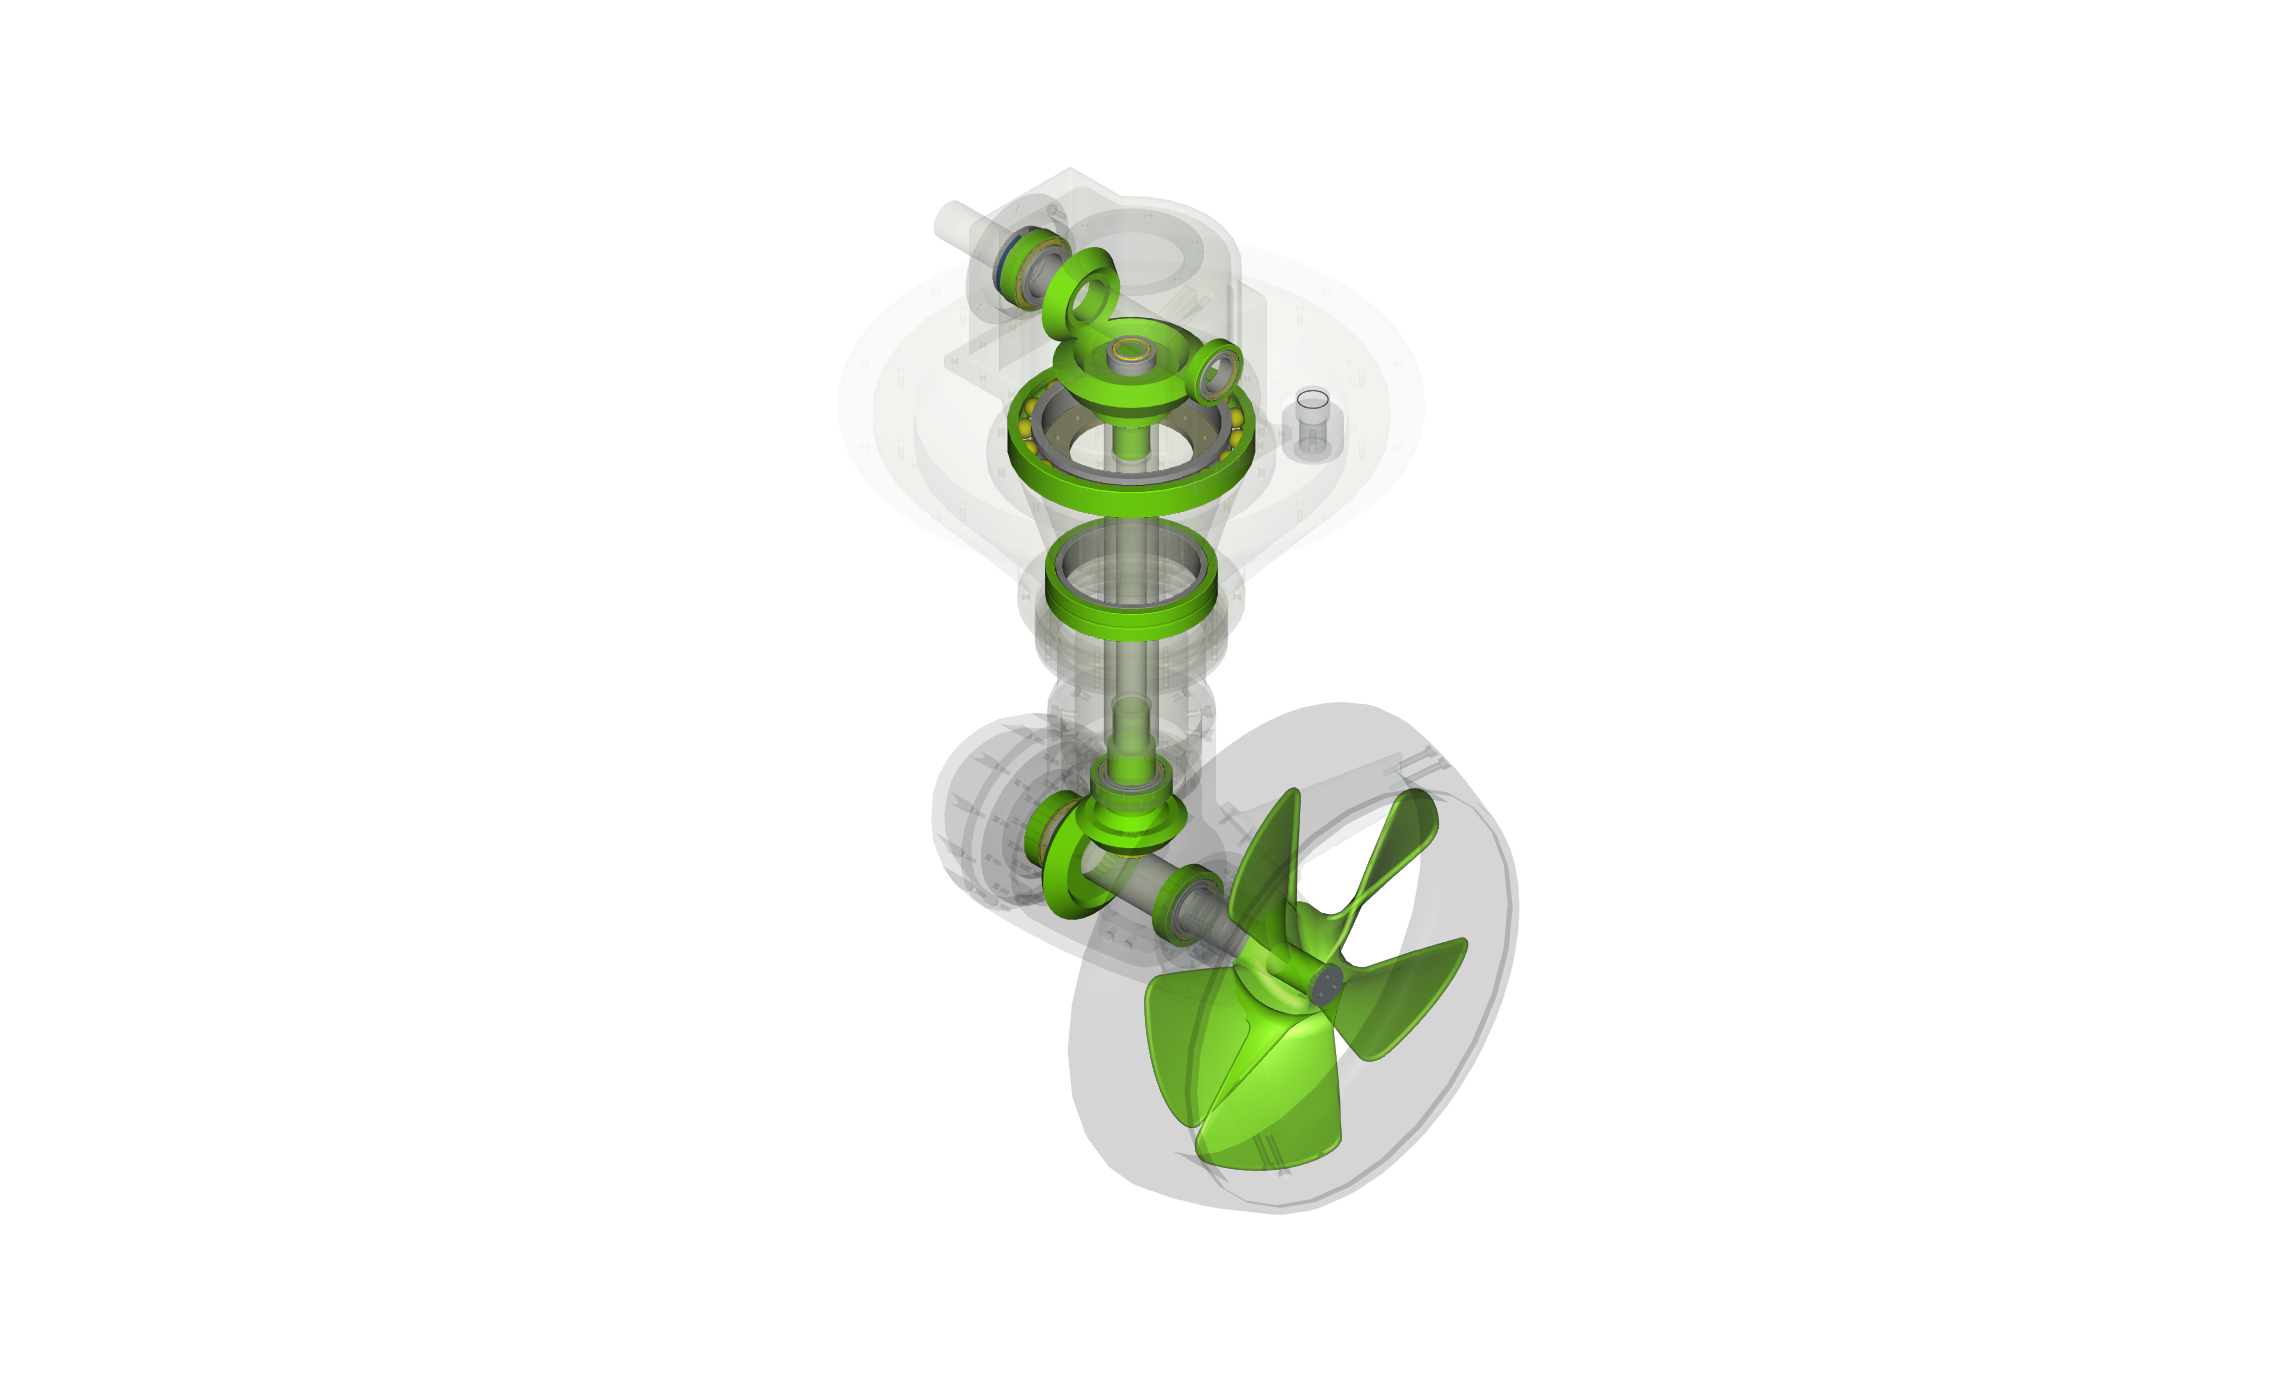
\includegraphics[width=0.3\linewidth]{thruster}
		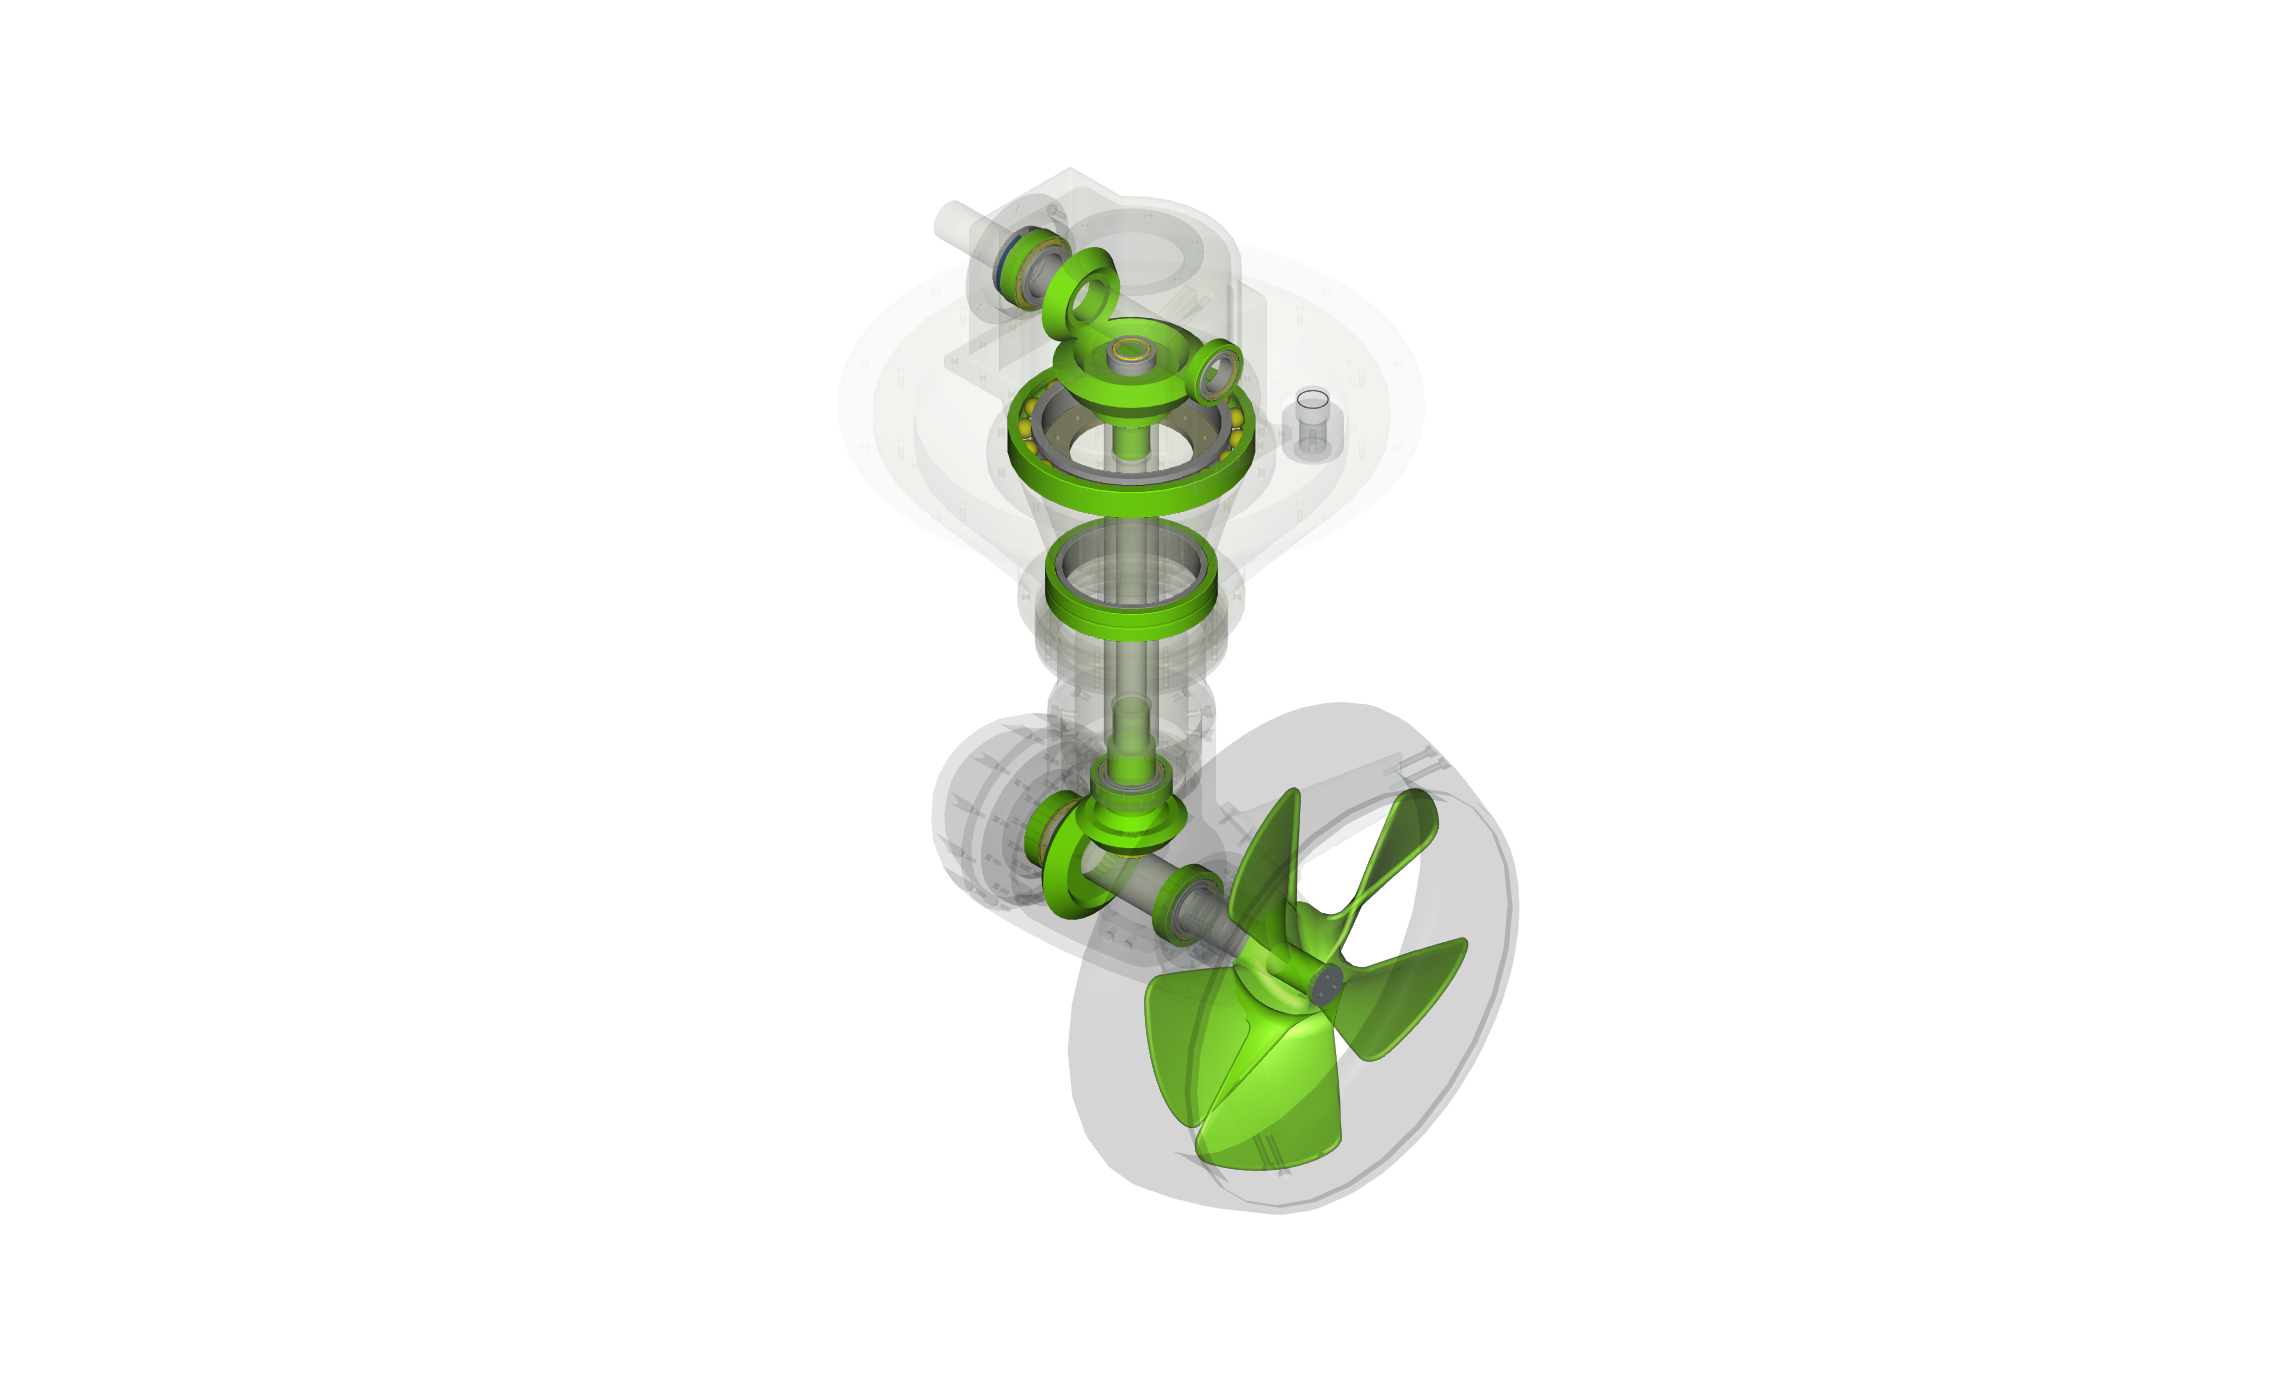
\includegraphics[width=0.3\linewidth]{thruster}
		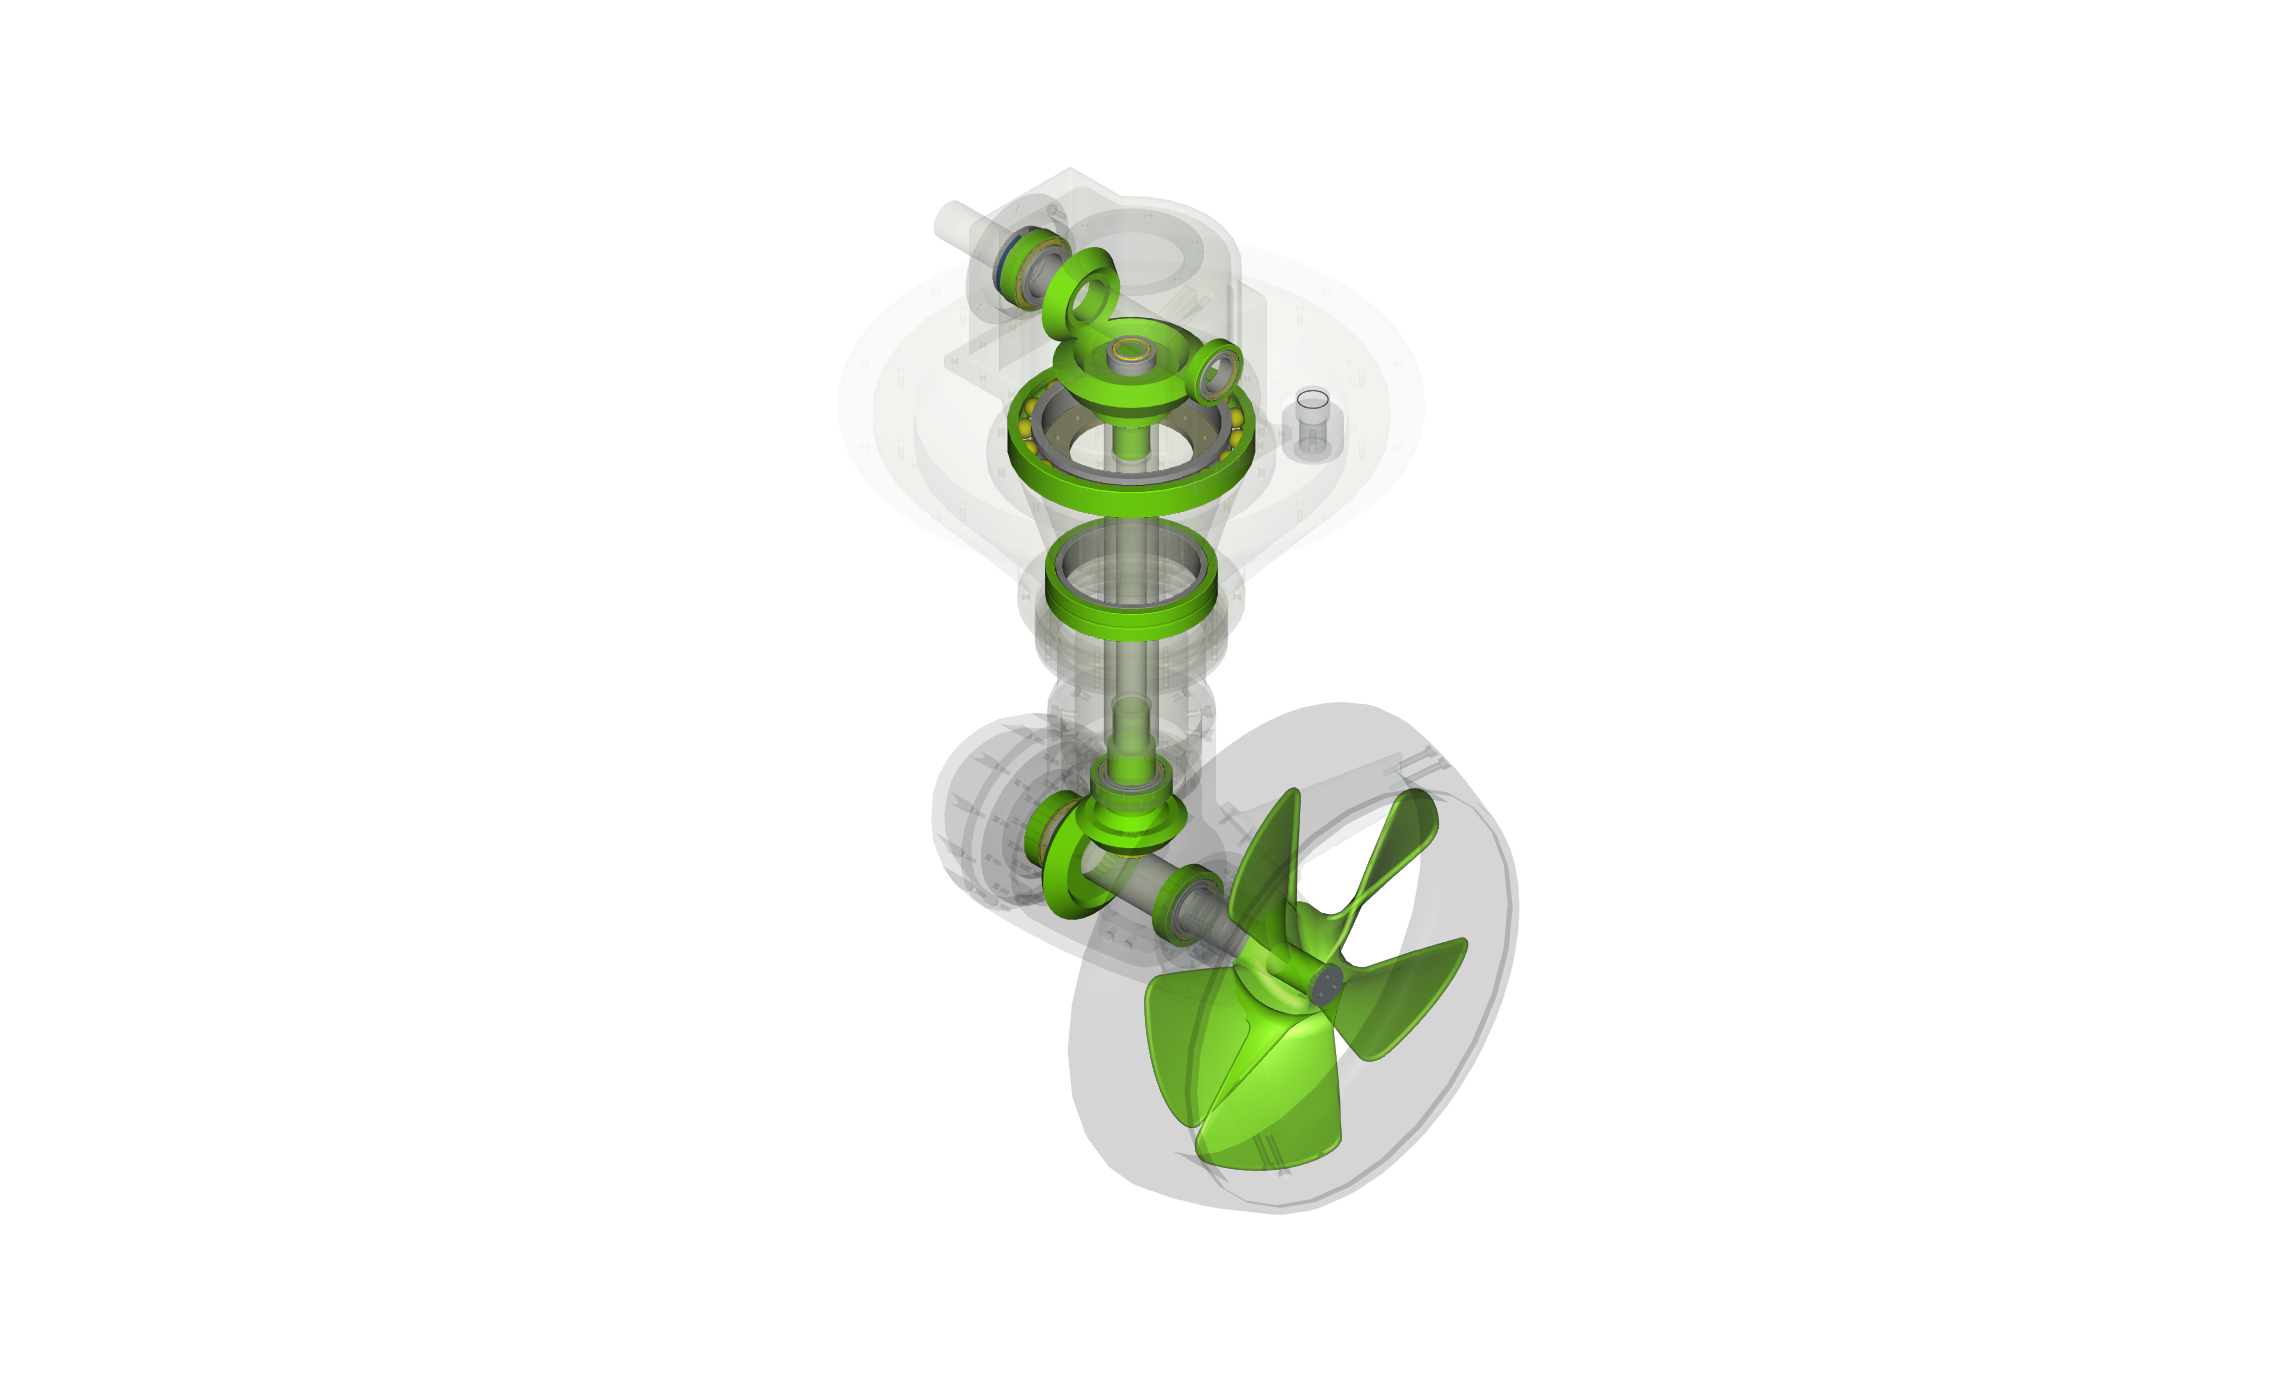
\includegraphics[width=0.3\linewidth]{thruster}
		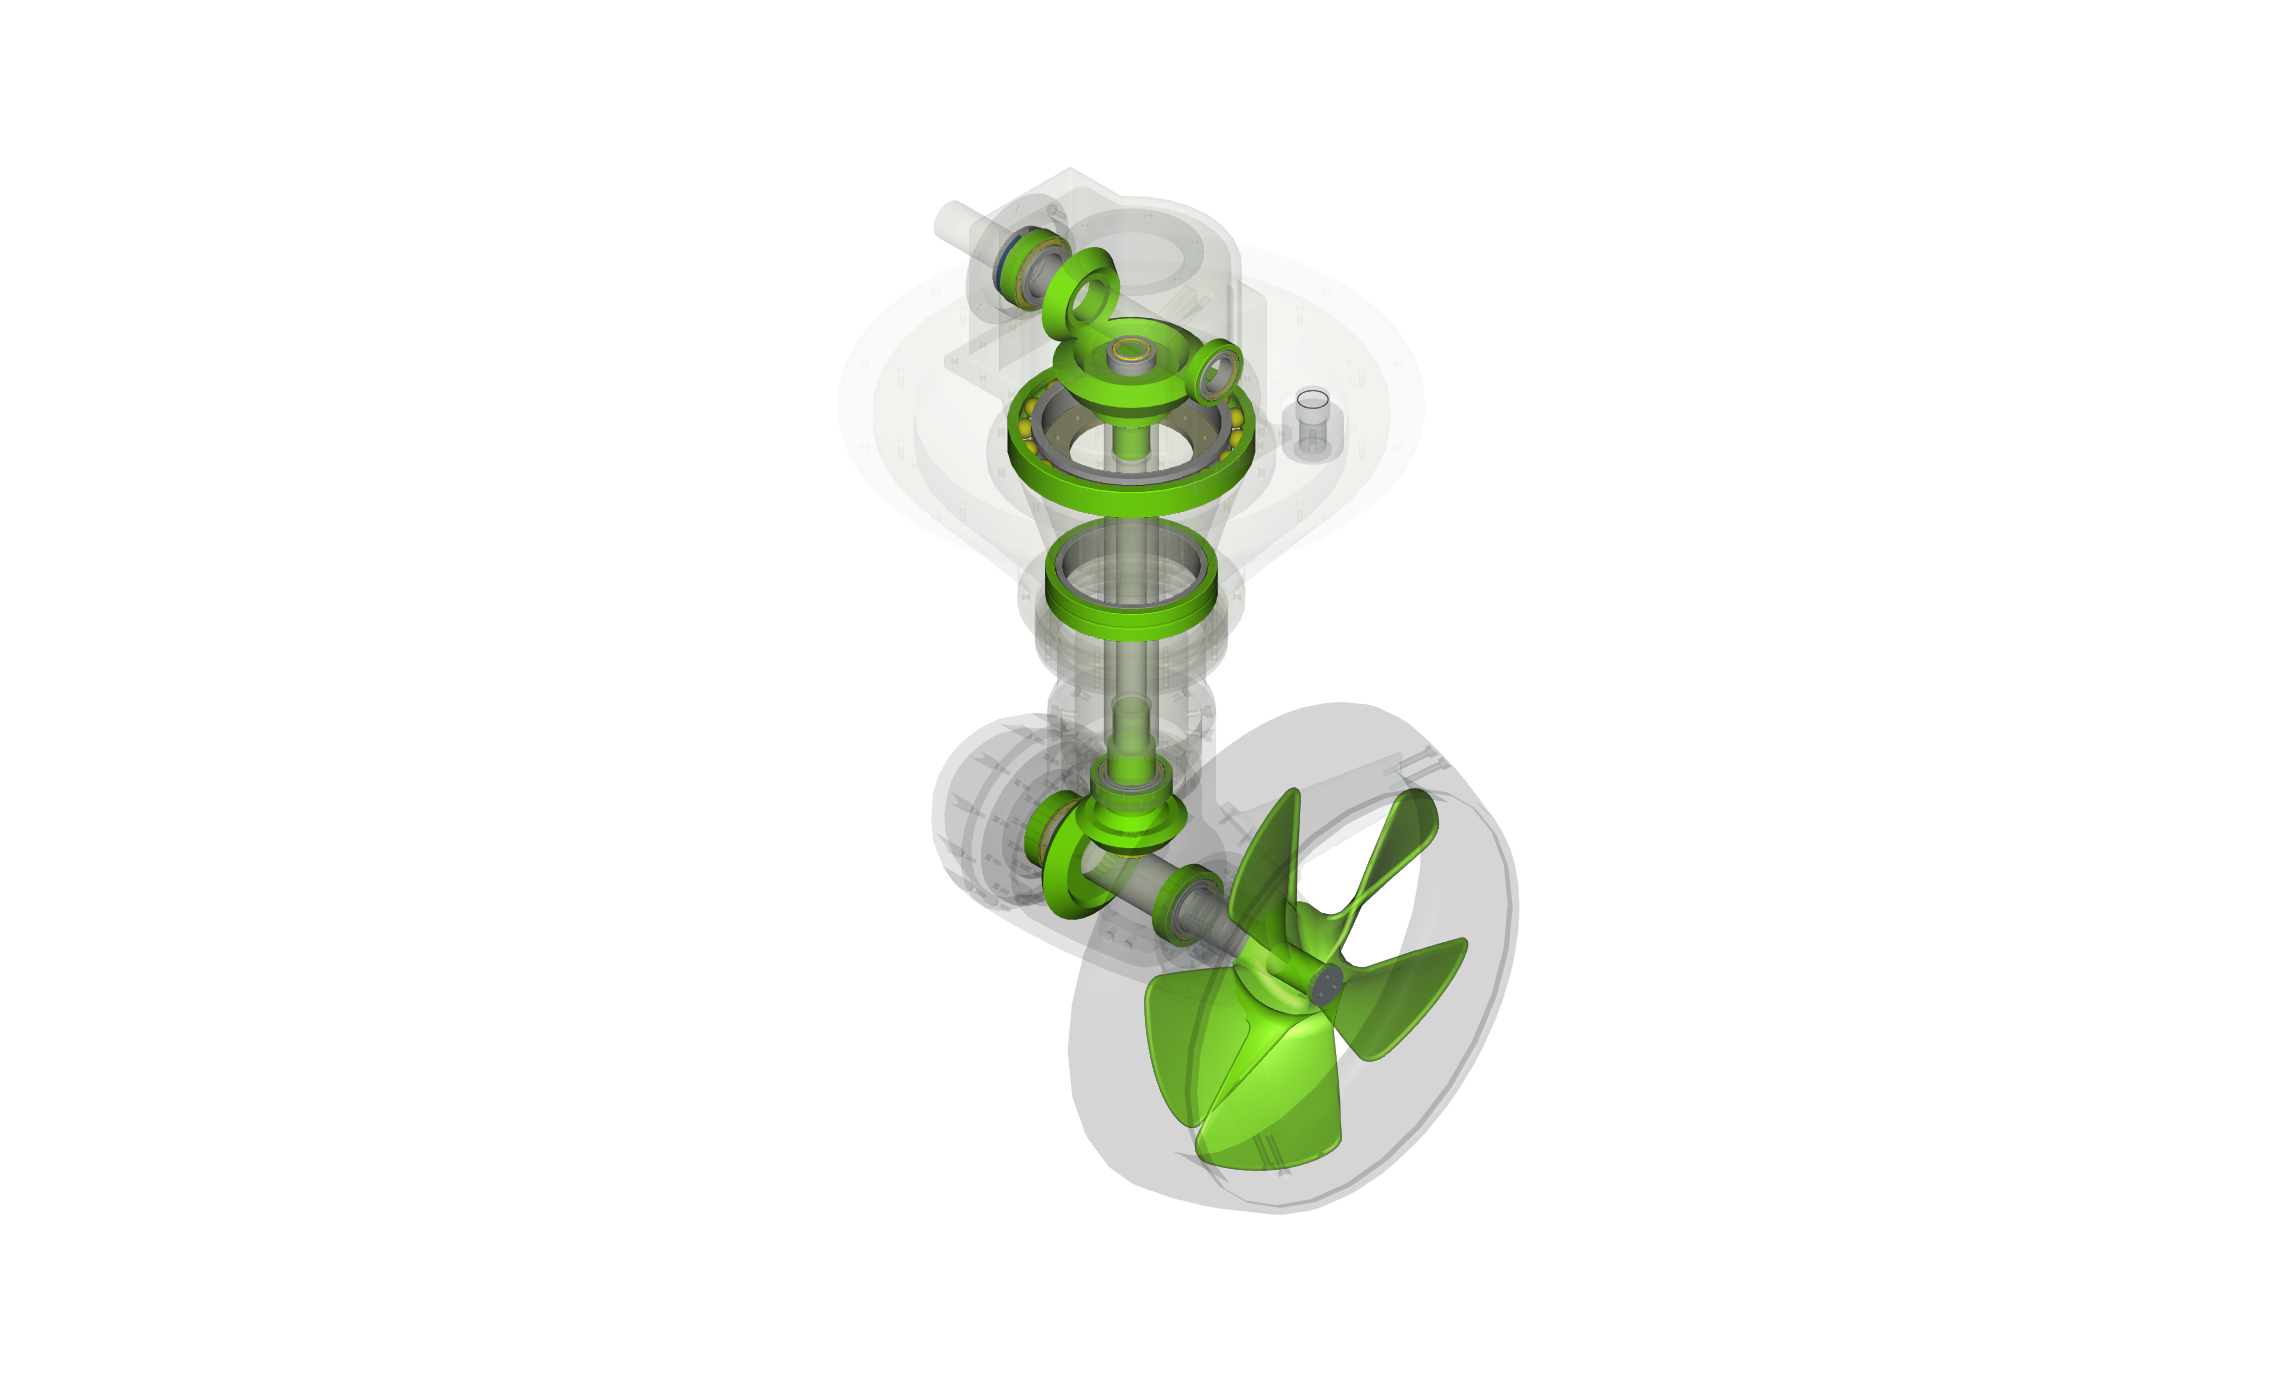
\includegraphics[width=0.3\linewidth]{thruster}
		%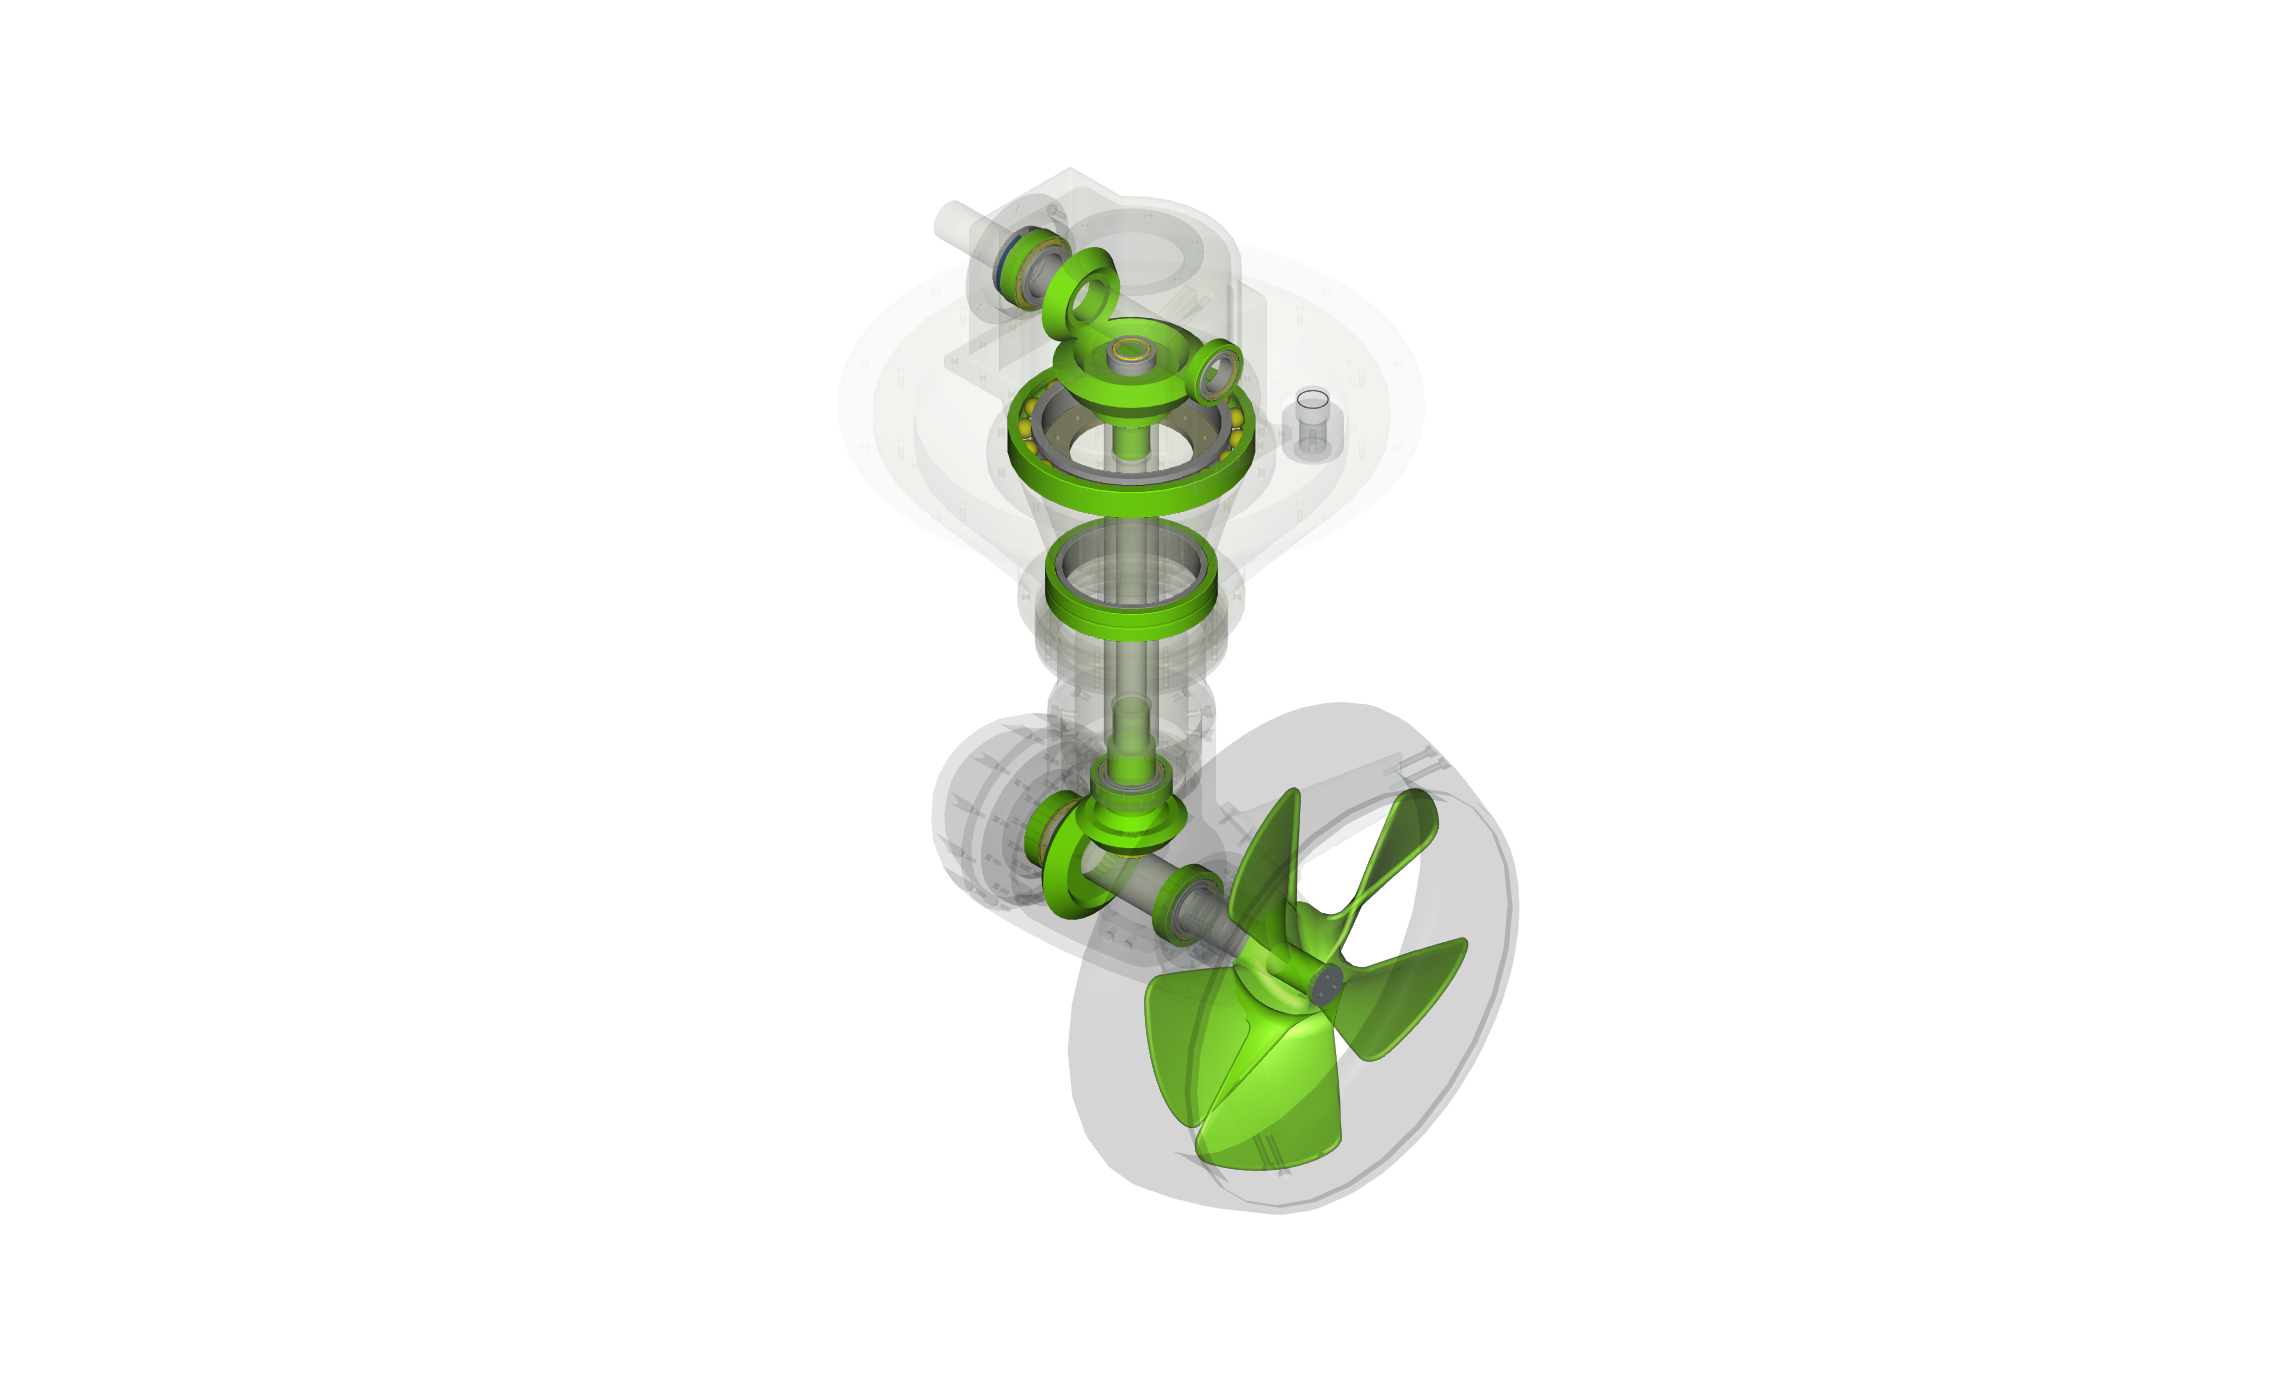
\includegraphics[width=0.3\linewidth]{thruster}
		%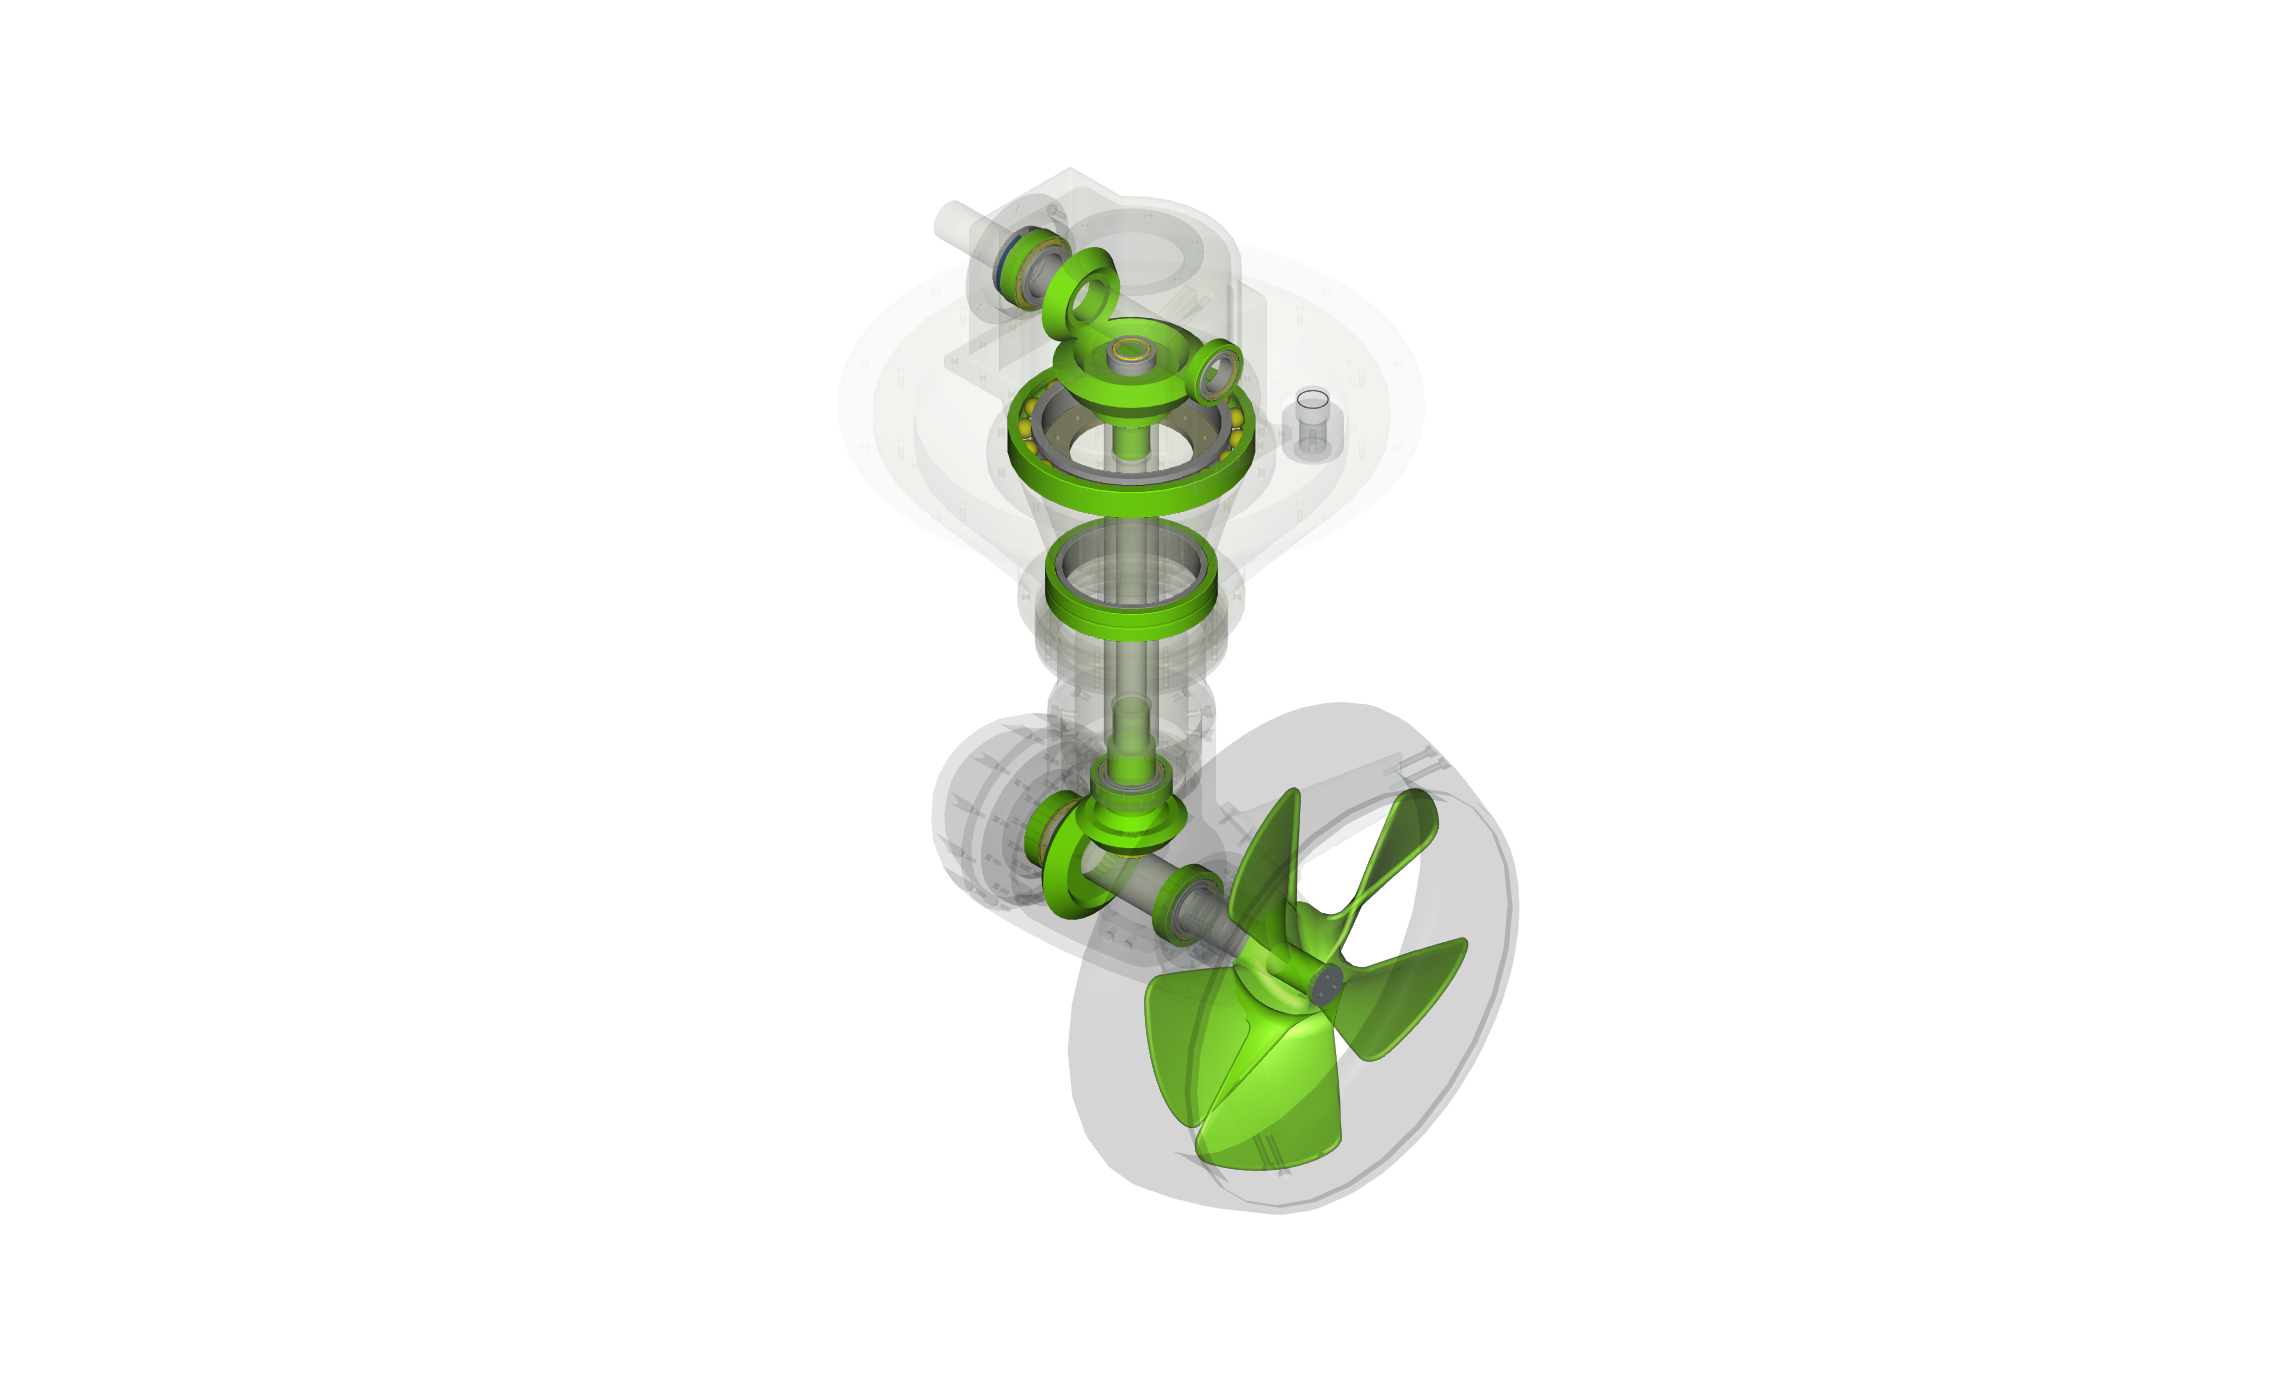
\includegraphics[width=0.3\linewidth]{thruster}
		%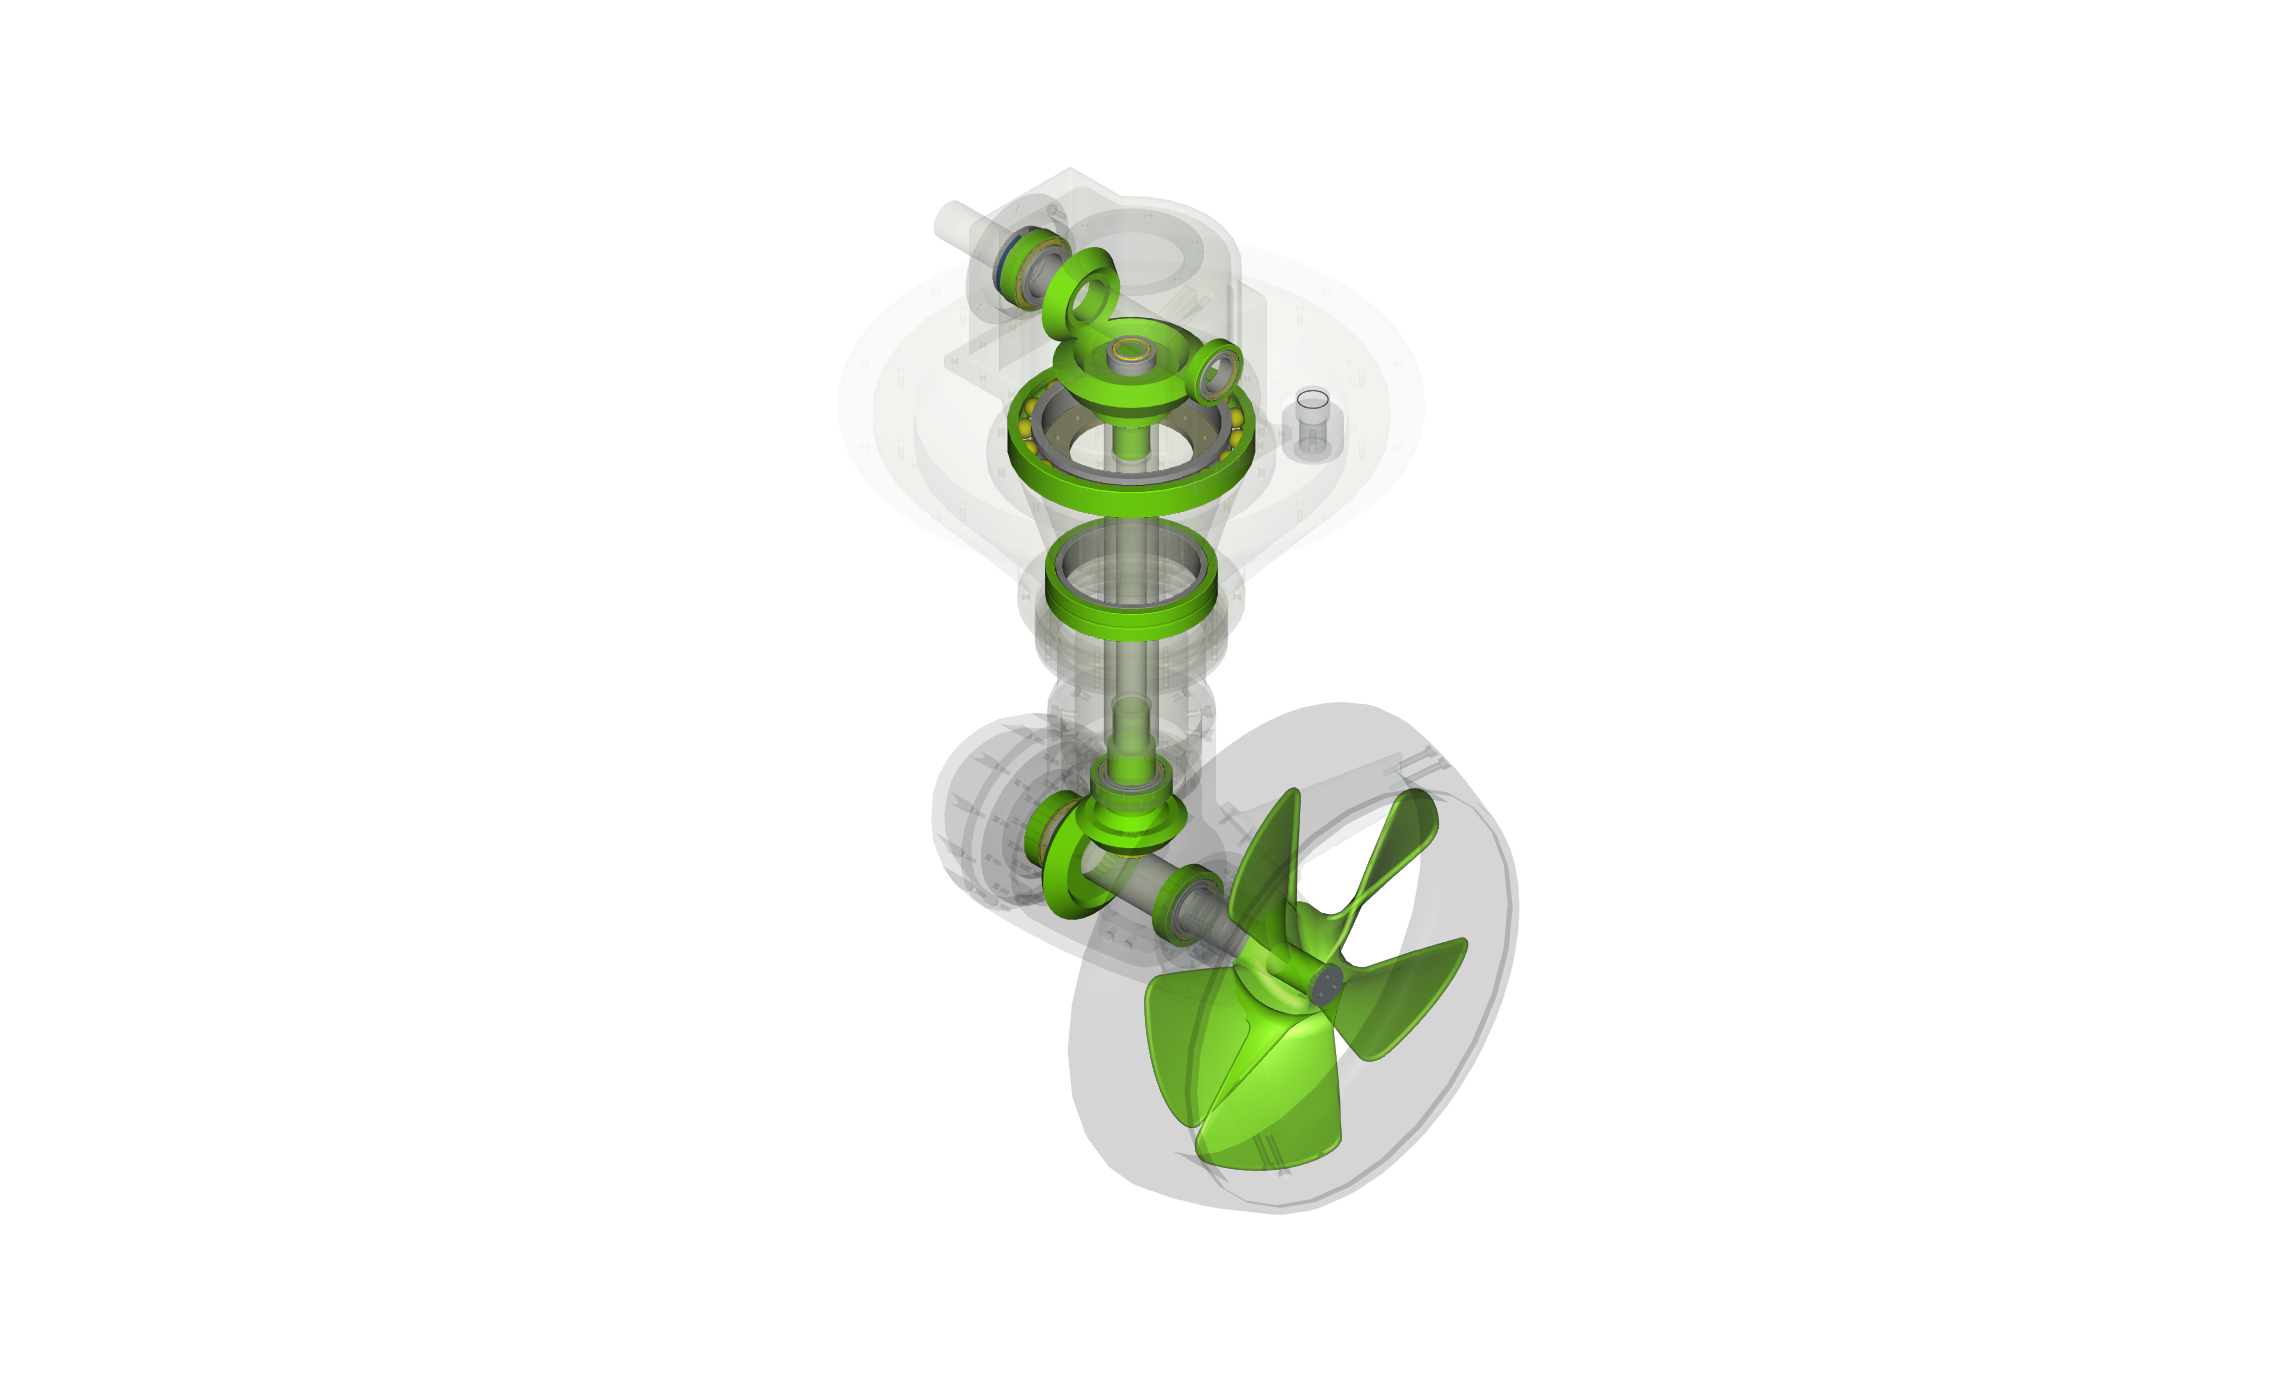
\includegraphics[width=0.3\linewidth]{thruster}
		%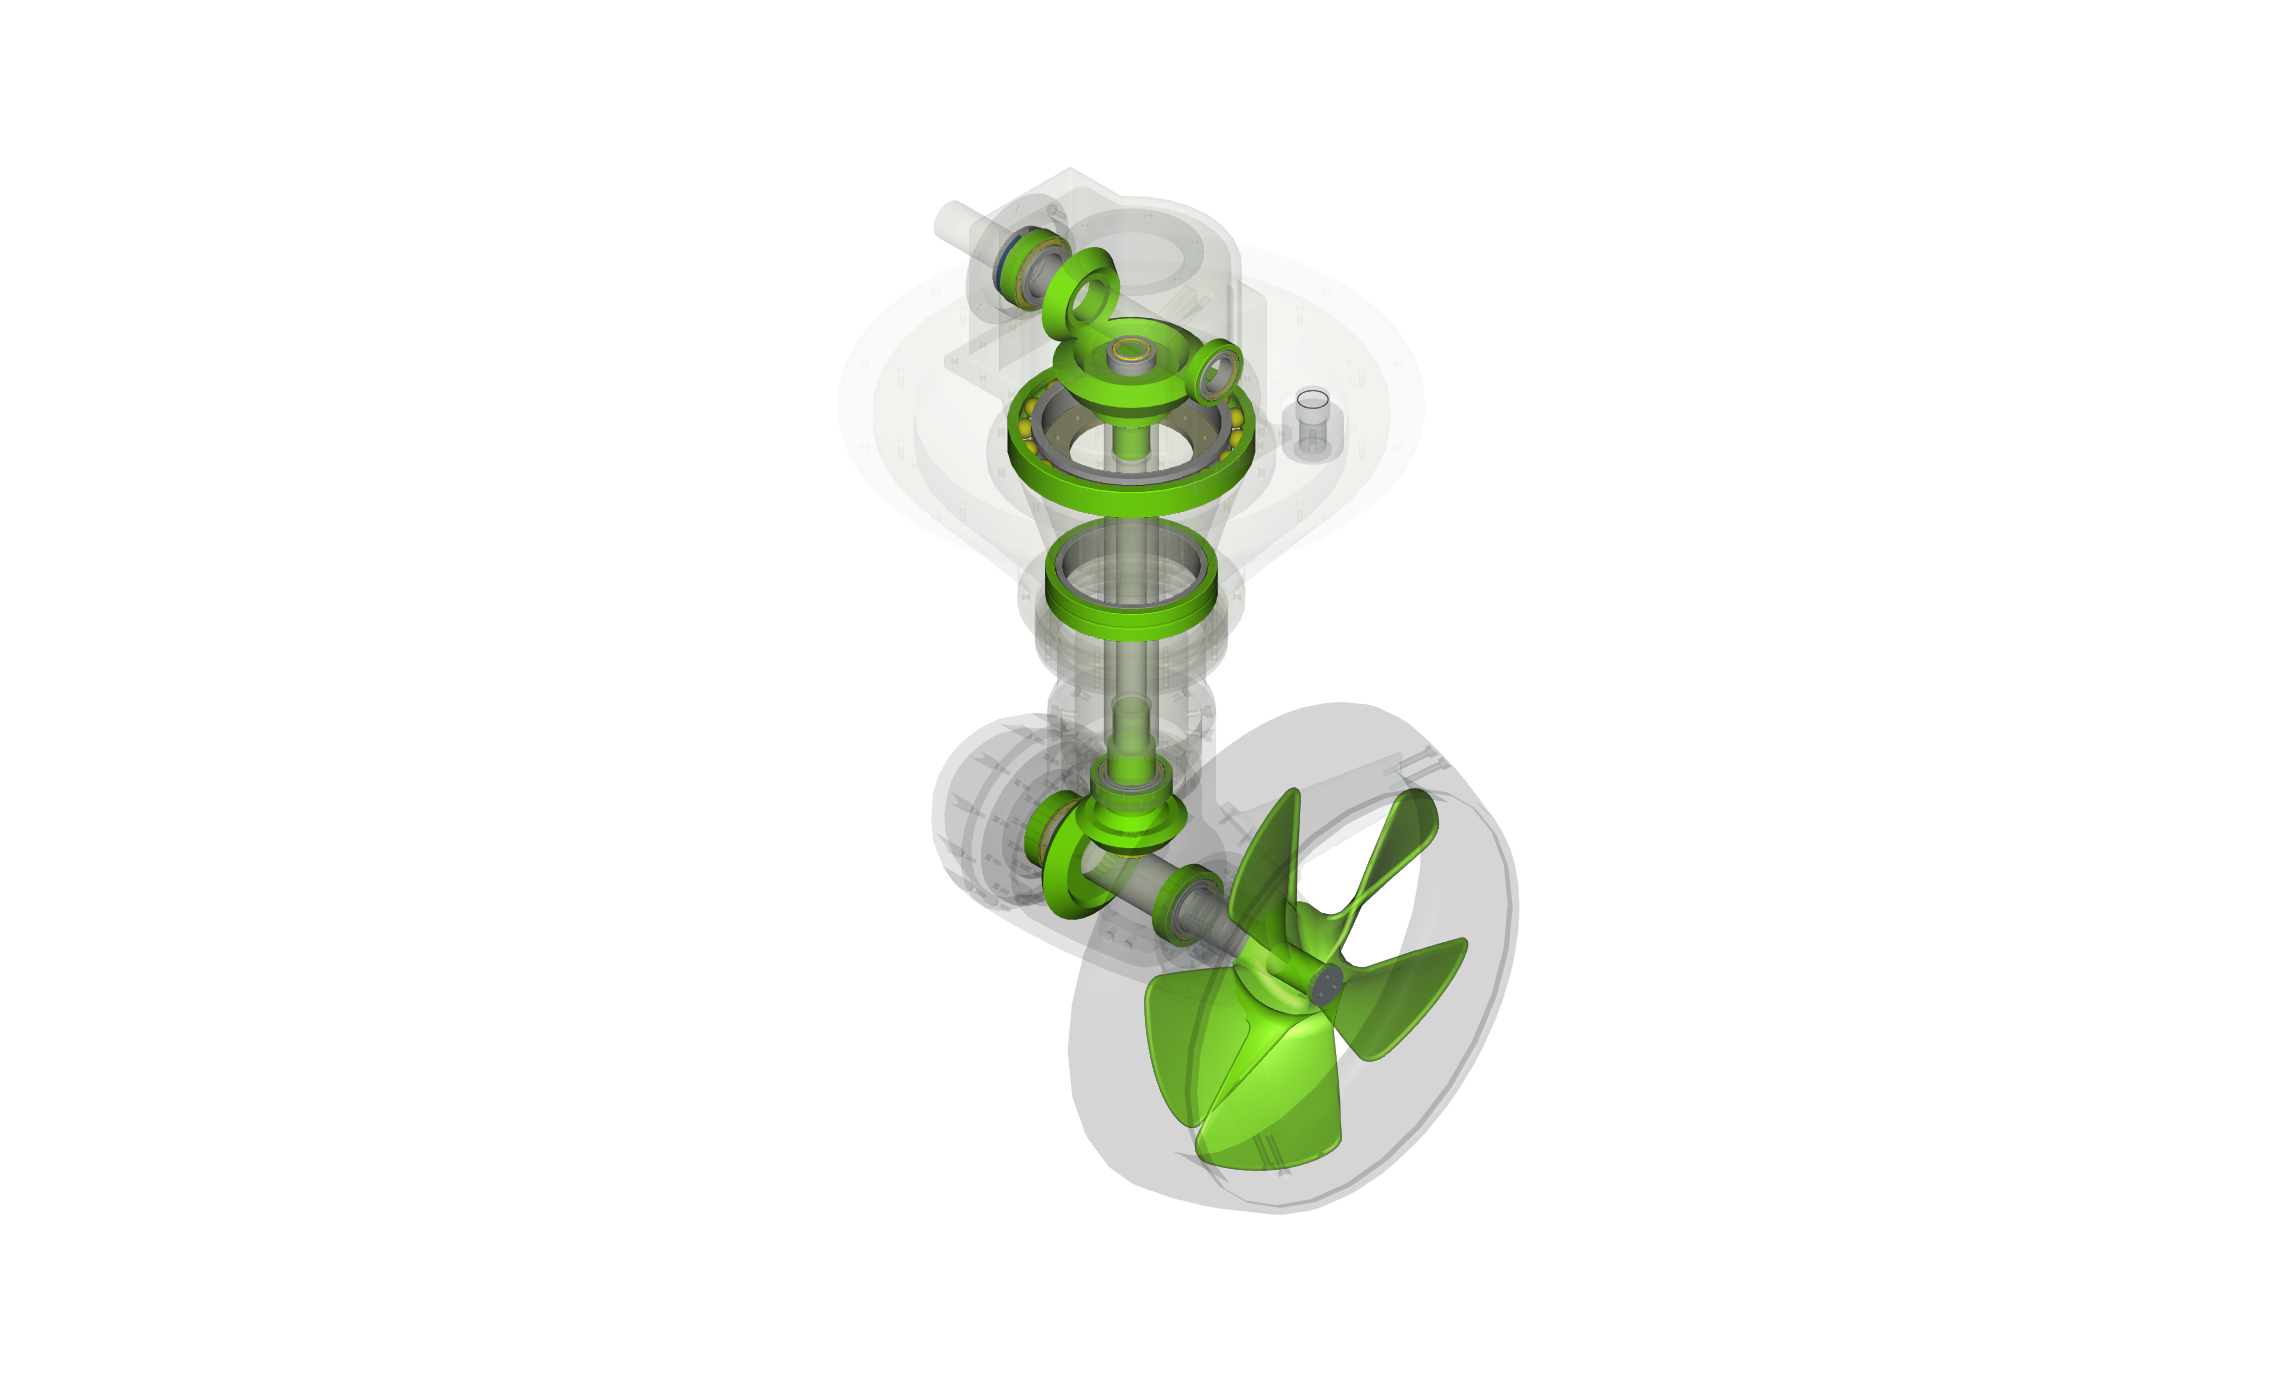
\includegraphics[width=0.3\linewidth]{thruster}
		%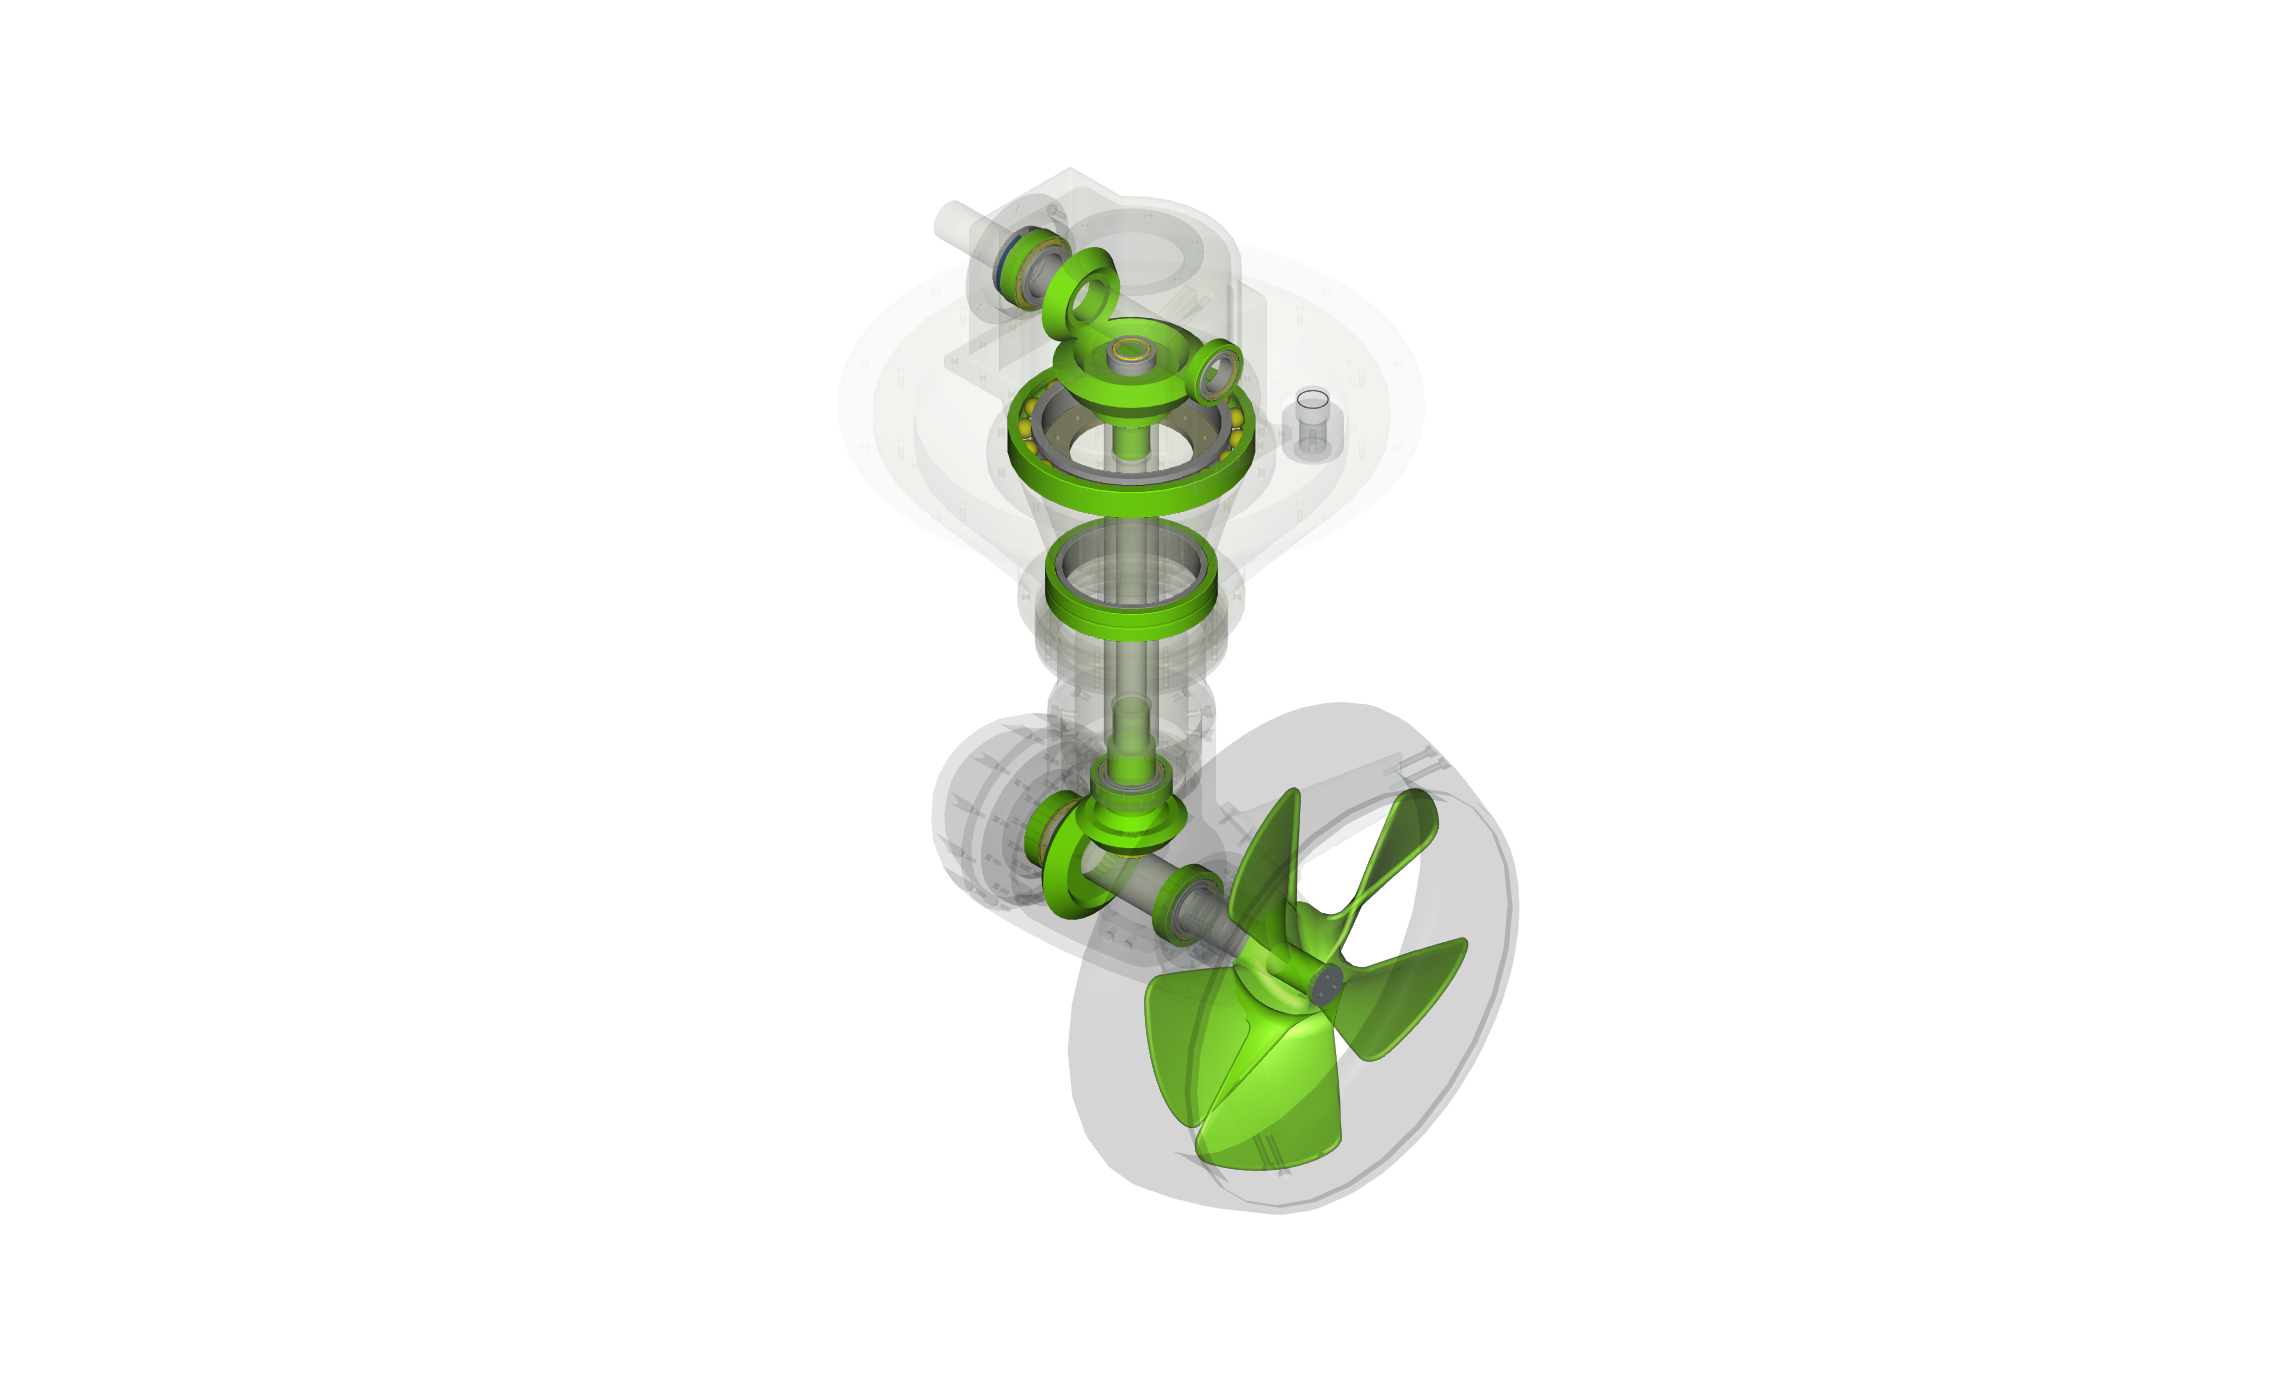
\includegraphics[width=0.3\linewidth]{thruster}
		%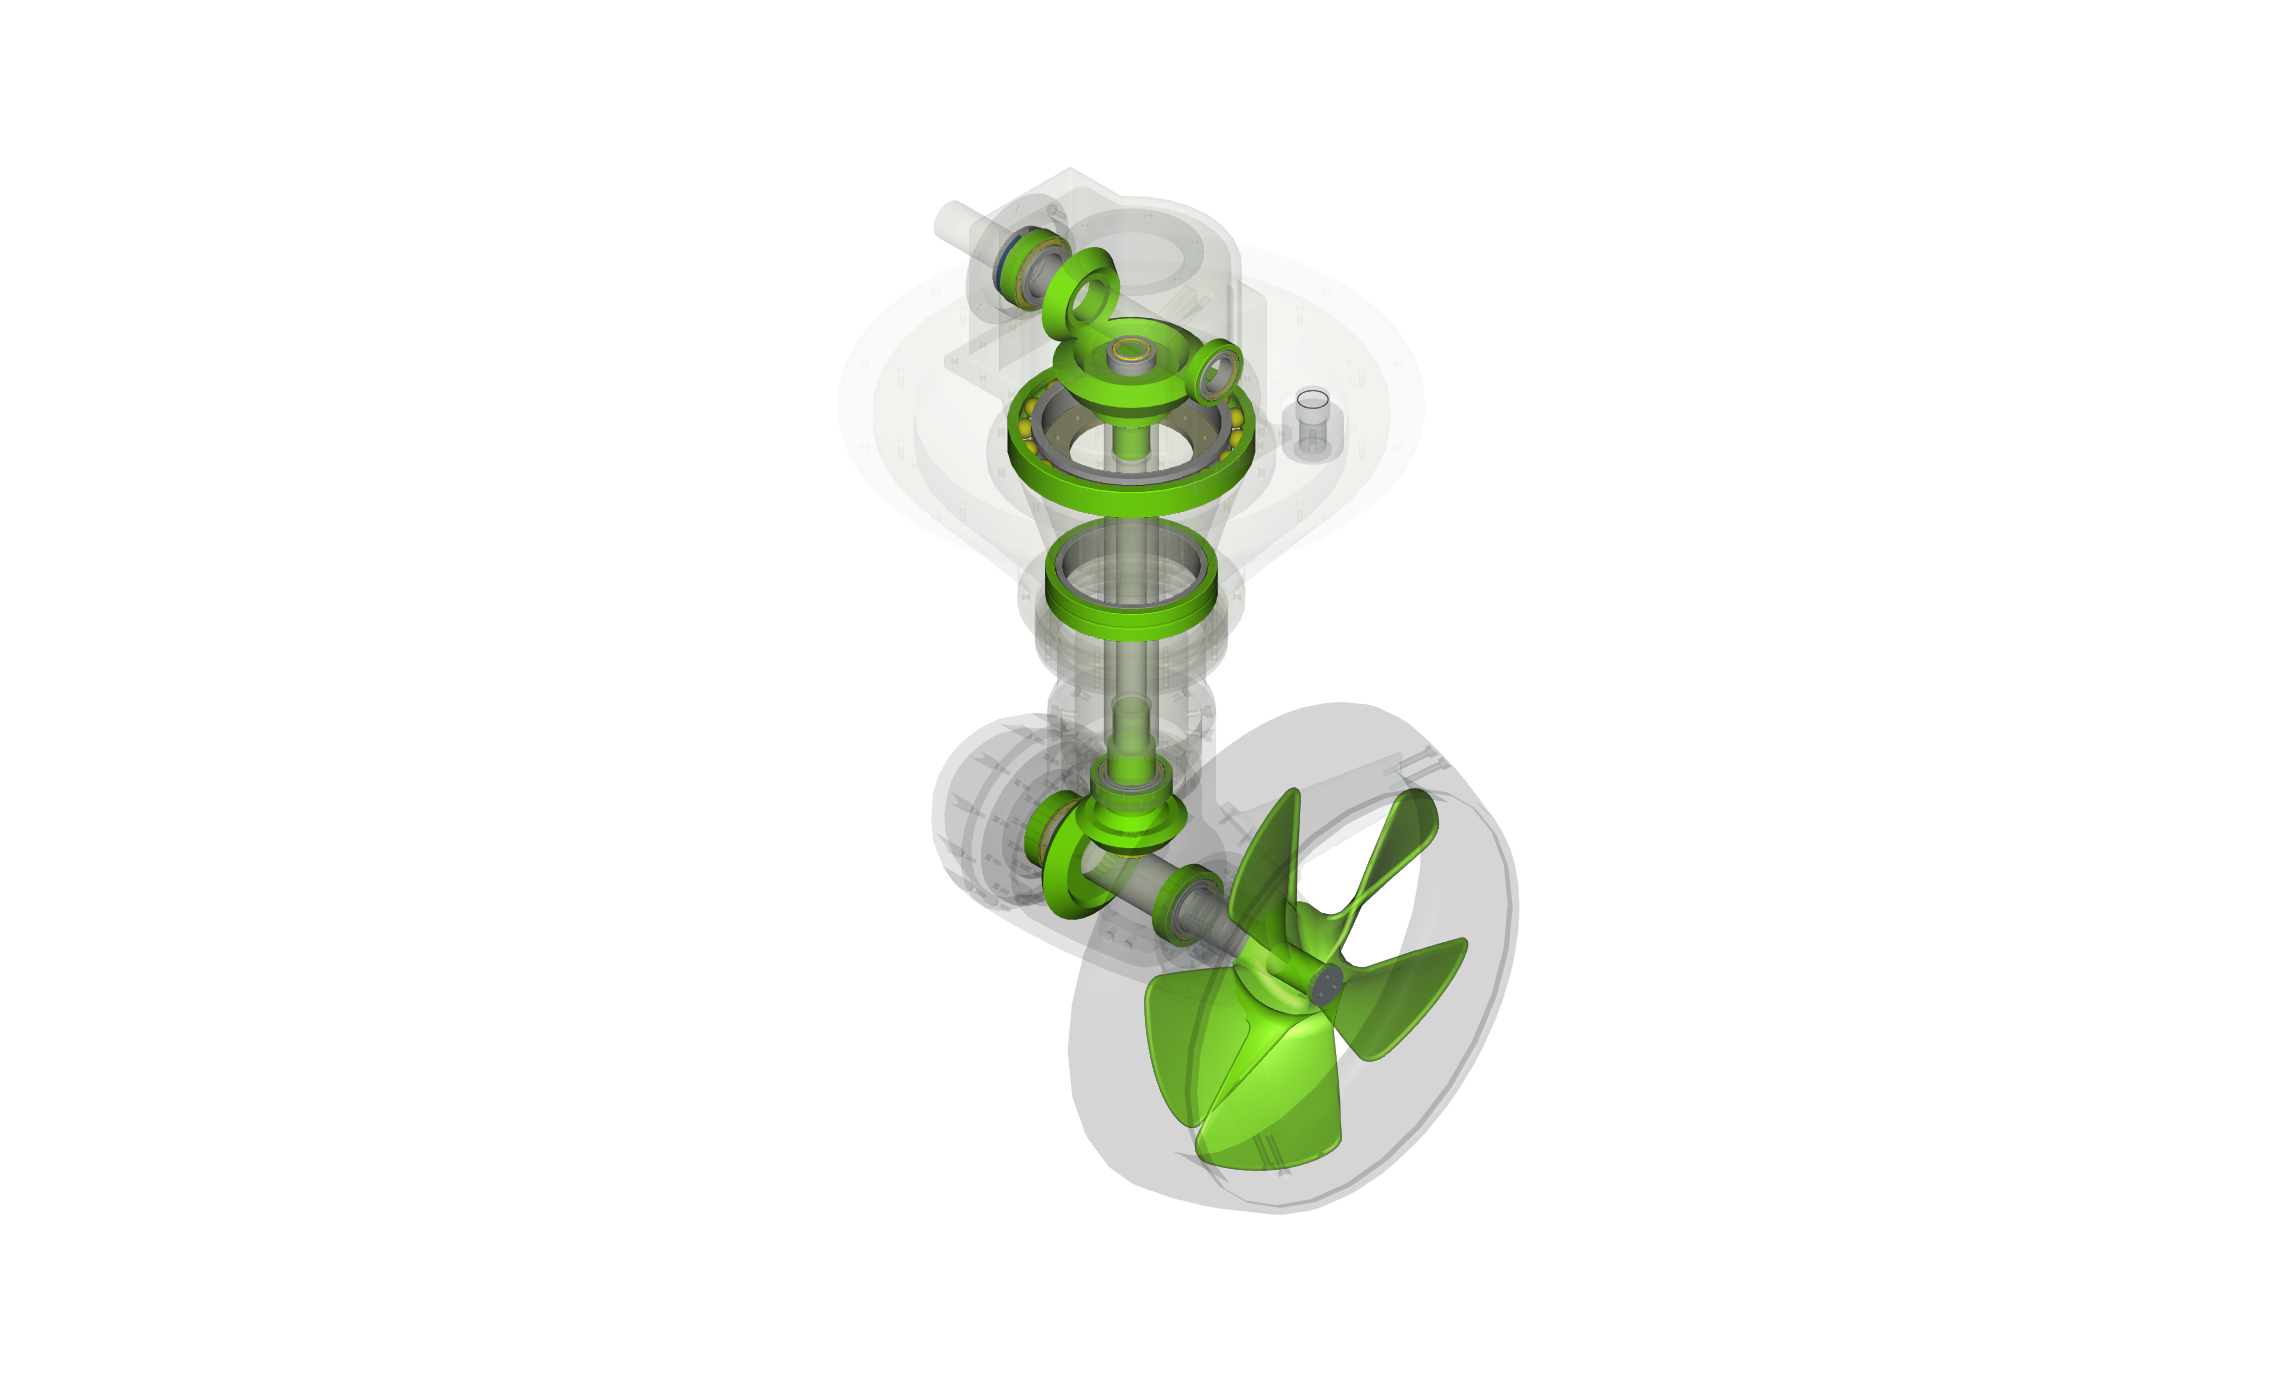
\includegraphics[width=0.3\linewidth]{thruster}
		%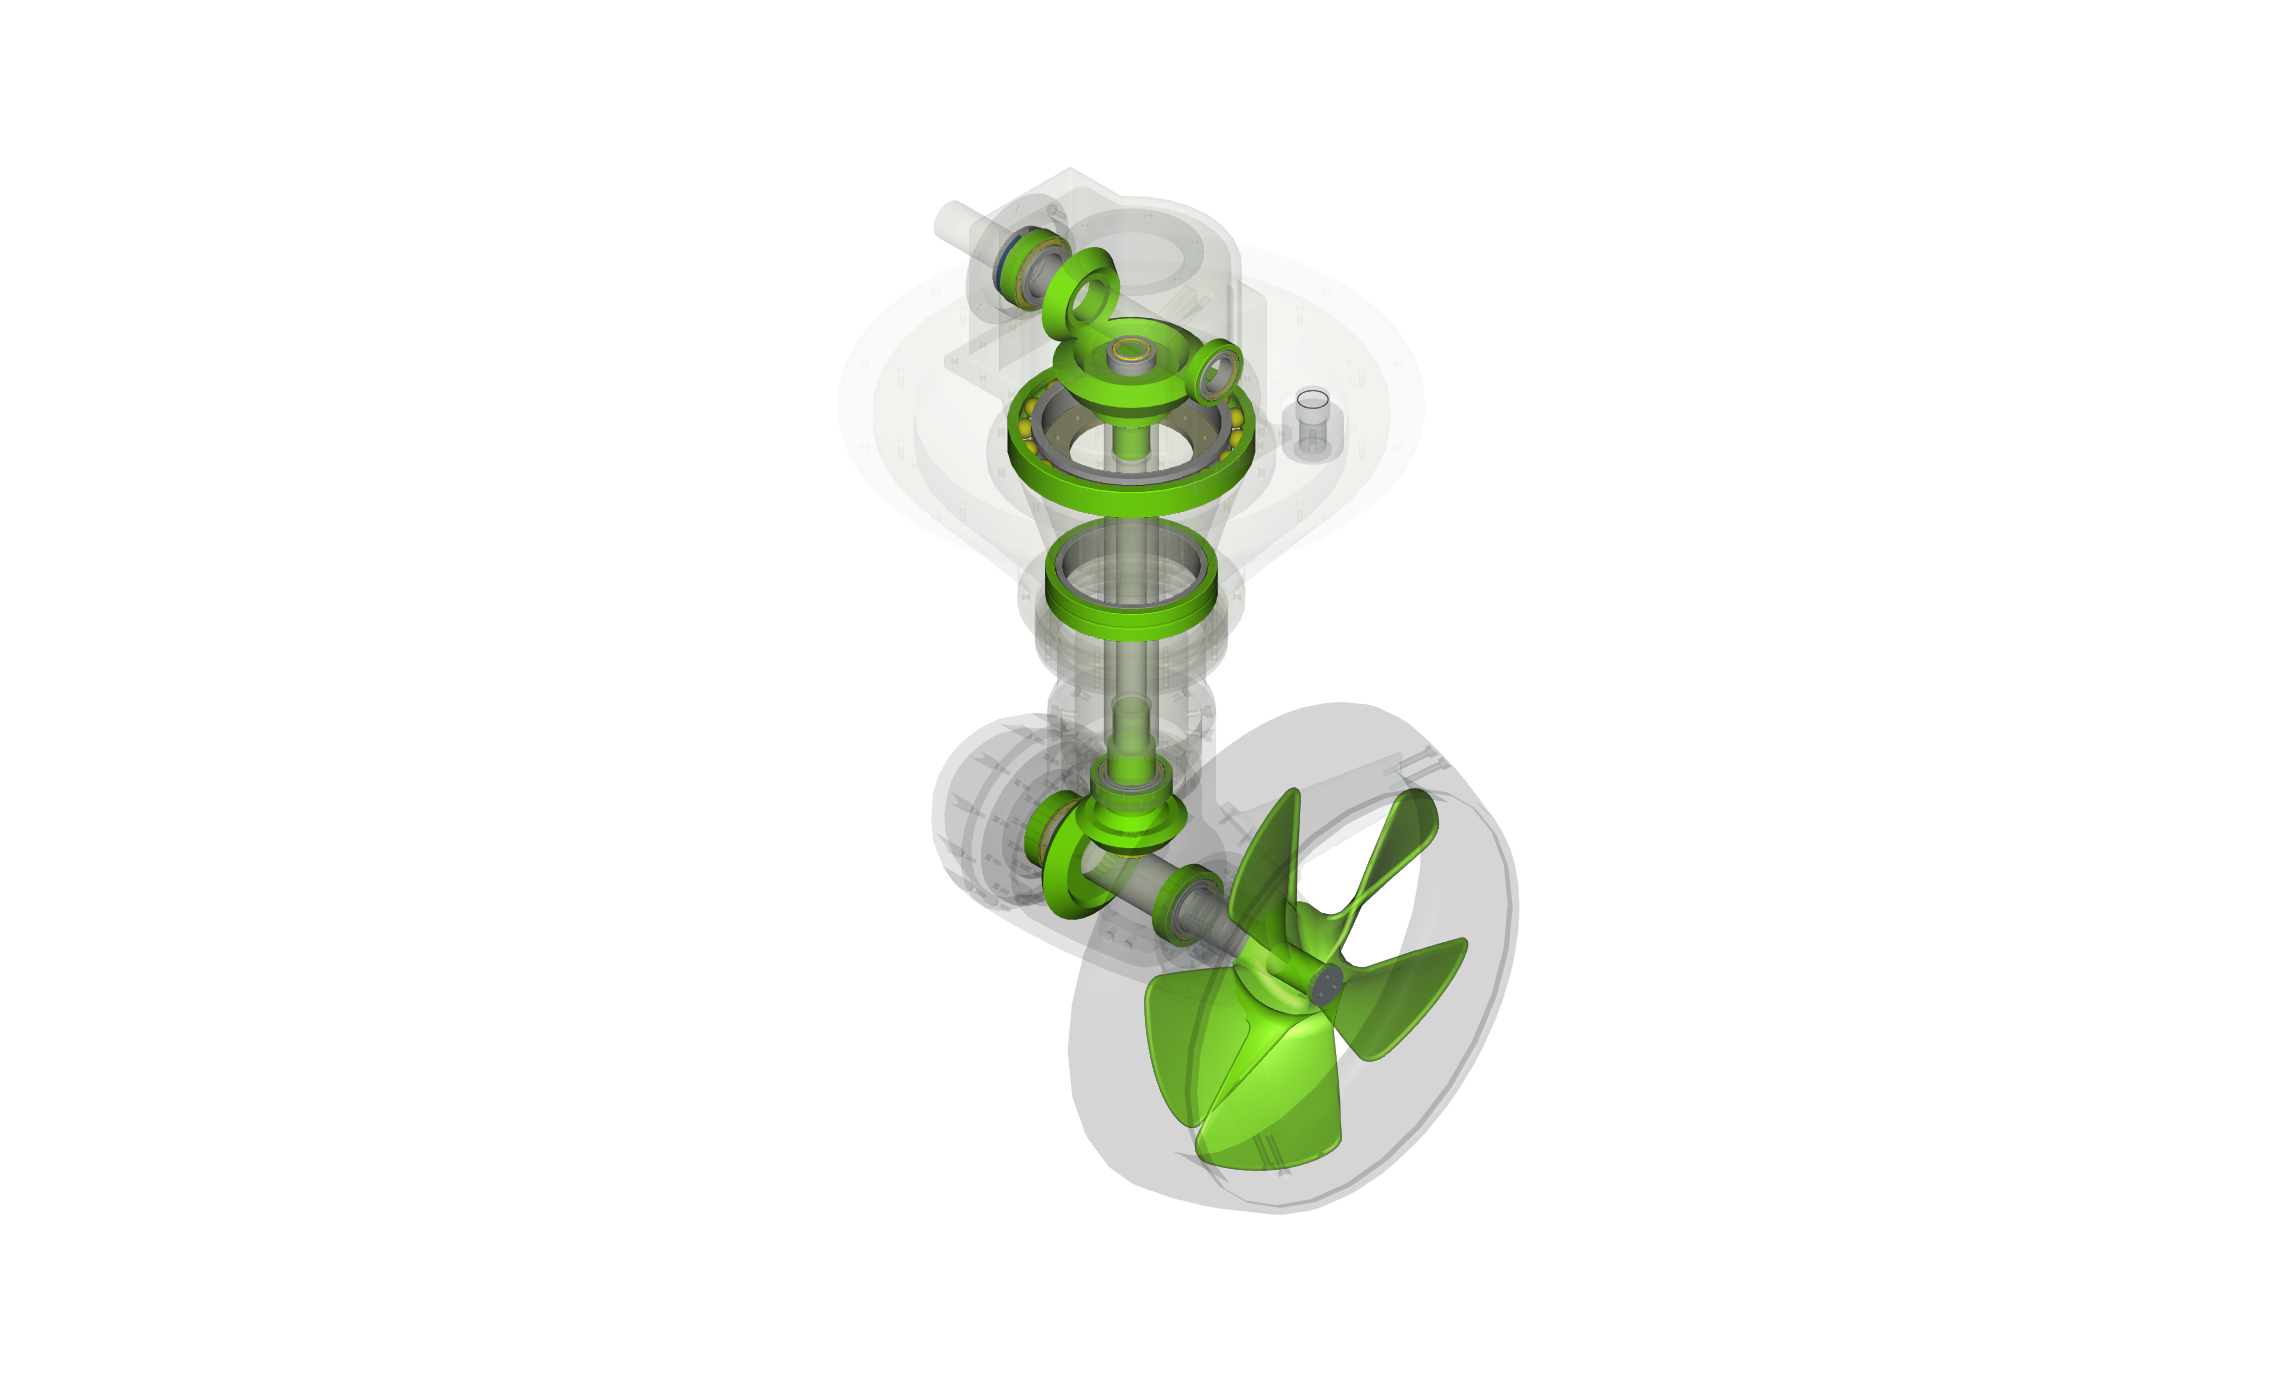
\includegraphics[width=0.3\linewidth]{thruster}
		%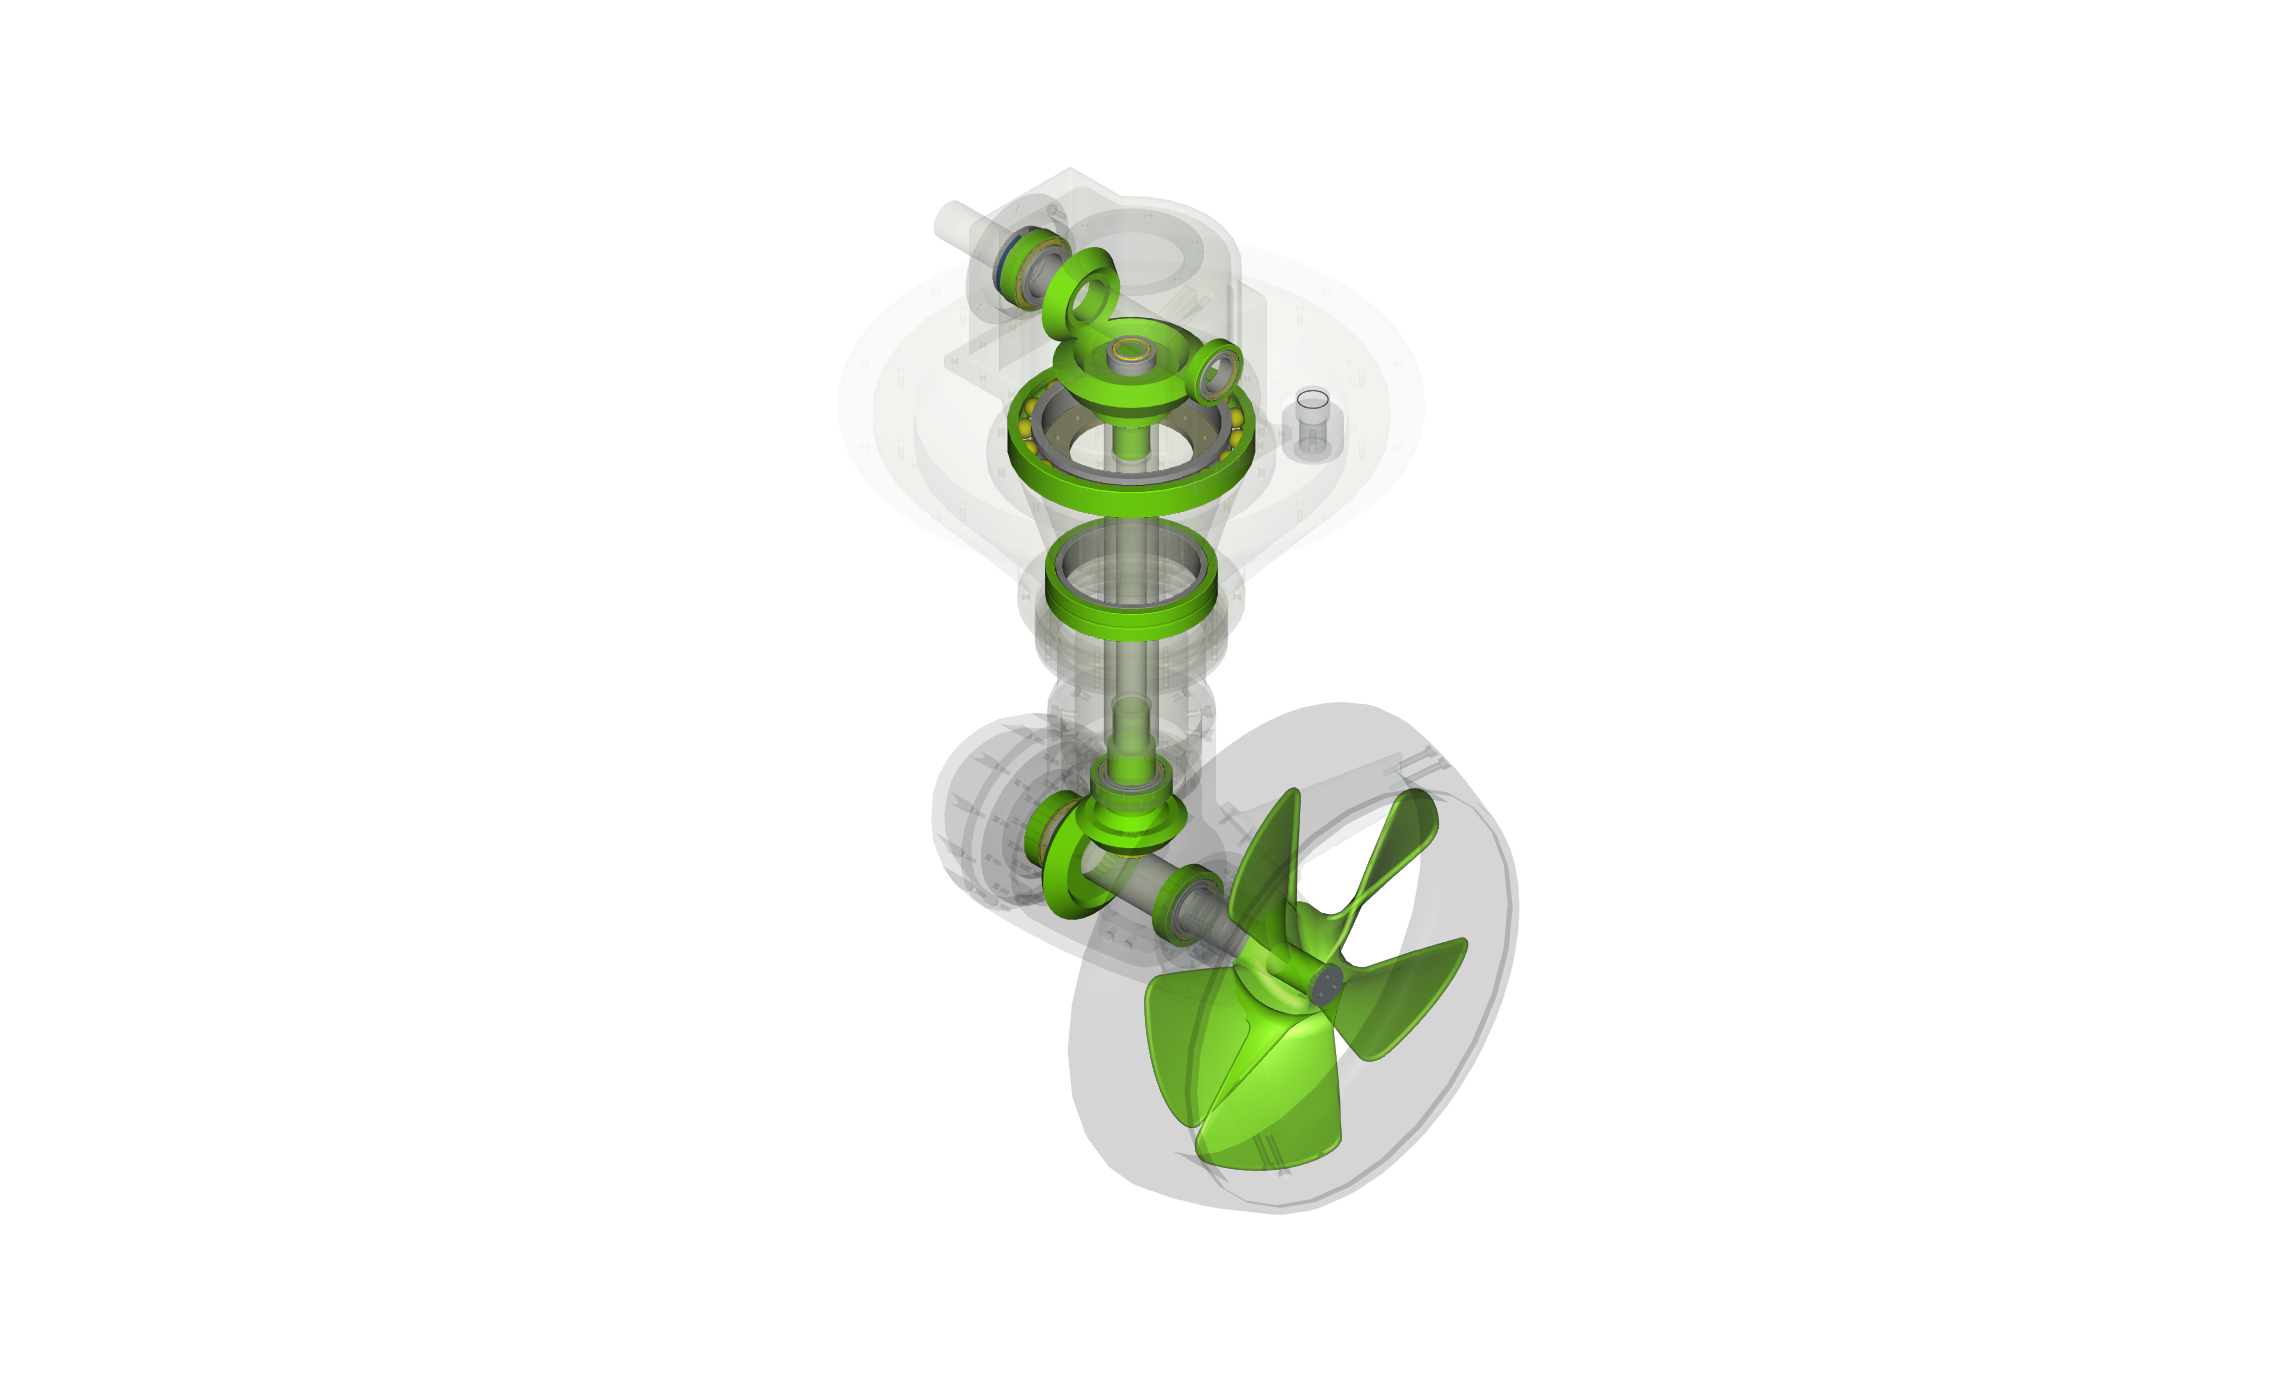
\includegraphics[width=0.3\linewidth]{thruster}
		%		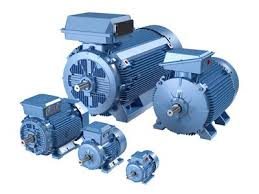
\includegraphics[width=0.2\linewidth]{motor1}
		%		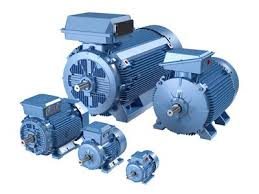
\includegraphics[width=0.2\linewidth]{motor1}
		%		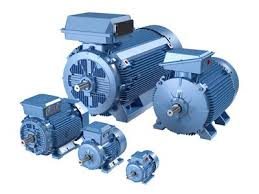
\includegraphics[width=0.2\linewidth]{motor1}
		%		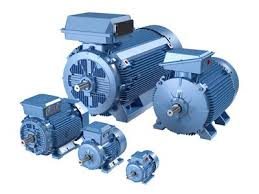
\includegraphics[width=0.2\linewidth]{motor1}
		%\caption{}
		%	\label{fig:datascience}
	\end{figure}
\end{frame}


%%%%%%%%%%%%%%%%%%%%%%%%%%%%%%%%%%%%%%%%%%%%%%%%%
\begin{frame}
	\frametitle{Data science for maintenance optimization}
		\begin{figure}[H]
			\centering
			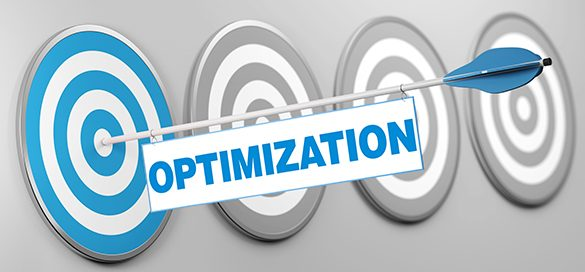
\includegraphics[width=0.5\linewidth]{optimization}
			%\caption{}
			%\label{fig:datascience}
		\end{figure}
	\begin{itemize}
		\item Part ordering
		\item Maintenance planing
		\item Production optimization
		\item Process optimization
		\item
	\end{itemize}
\end{frame}

%%%%%%%%%%%%%%%%%%%%%%%%%%%%%%%%%%%%%%%%%%%%%%%%%
\begin{frame}
	\frametitle{Data science in predictive maintenance: \textcolor{orange}{Bearings fault detection}}
	\begin{figure}[H]
		\centering
		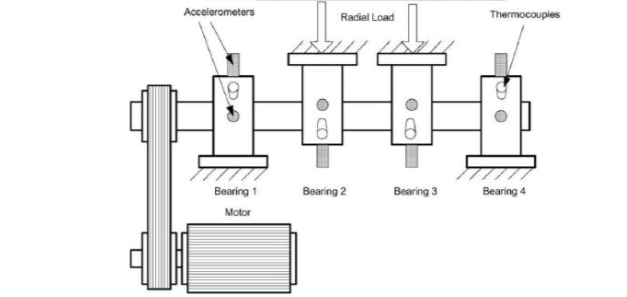
\includegraphics[width=0.6\linewidth]{experiment}
		
\includegraphics[width=0.05\linewidth]{arrow}
		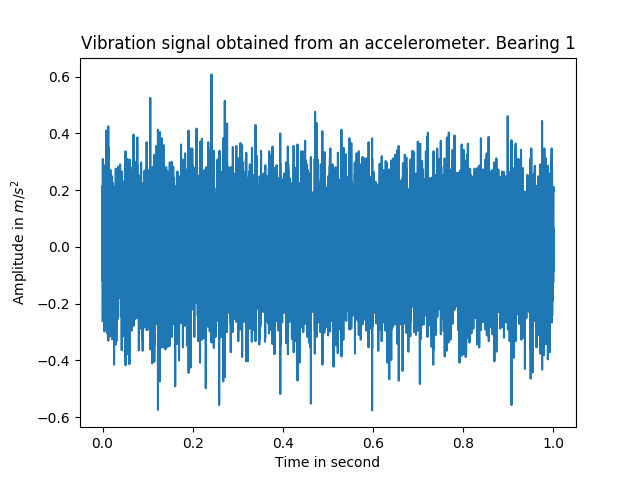
\includegraphics[width=0.3\linewidth]{data}
		%\caption{}
		%\label{fig:datascience}
	\end{figure}
\end{frame}
%%%%%%%%%%%%%%%%%%%%%%%%%%%%%%%%%%%%%%%%%%%%%%%%%%%



%%%%%%%%%%%%%%%%%%%%%%%%%%%%%%%%%%%%%%%%%%%%%%%%%%%%%%%%%%%%%%%%%%%%%%%%%%%%%%%%%%%%



%%%%%%%%%%%%%%%%%%%%%%%%%%%%%%%%%%%%%%%%%%%%%%%%%%%%%%%%%%%%%%%%%%%%%%%%%%%%%
\begin{frame}
	\frametitle{Data science in predictive maintenance: \textcolor{orange}{Machine health index}}
	\begin{figure}[H]
		\centering
		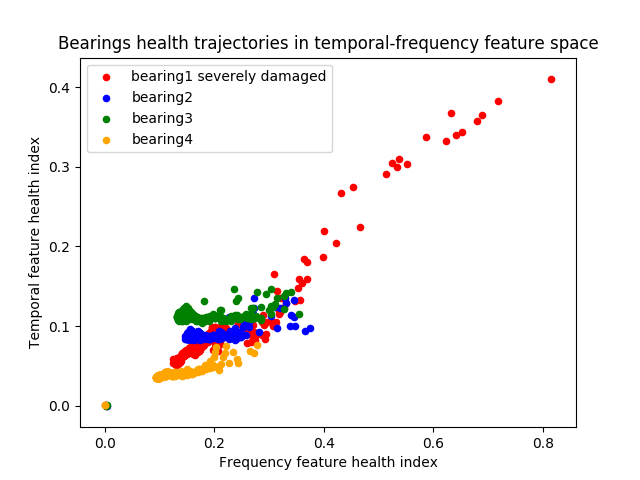
\includegraphics[width=0.5\linewidth]{health_plot}
		%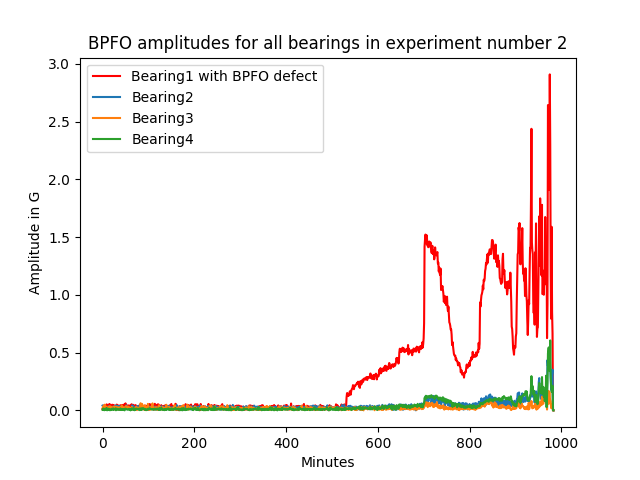
\includegraphics[width=0.4\linewidth]{bpfo}
		%\caption{}
		%\label{fig:datascience}
	\end{figure}
\end{frame}



%%%%%%%%%%%%%%%%%%%%%%%%%%%%%%%%%%%%%%%%%%%%%%%%%%%%%%%%%%%%%%%%%%%%%%%%%%%%%%
\begin{frame}
	\frametitle{Data science in predictive maintenance: \textcolor{orange}{Machine learning}}
	\begin{figure}[H]
		\centering
		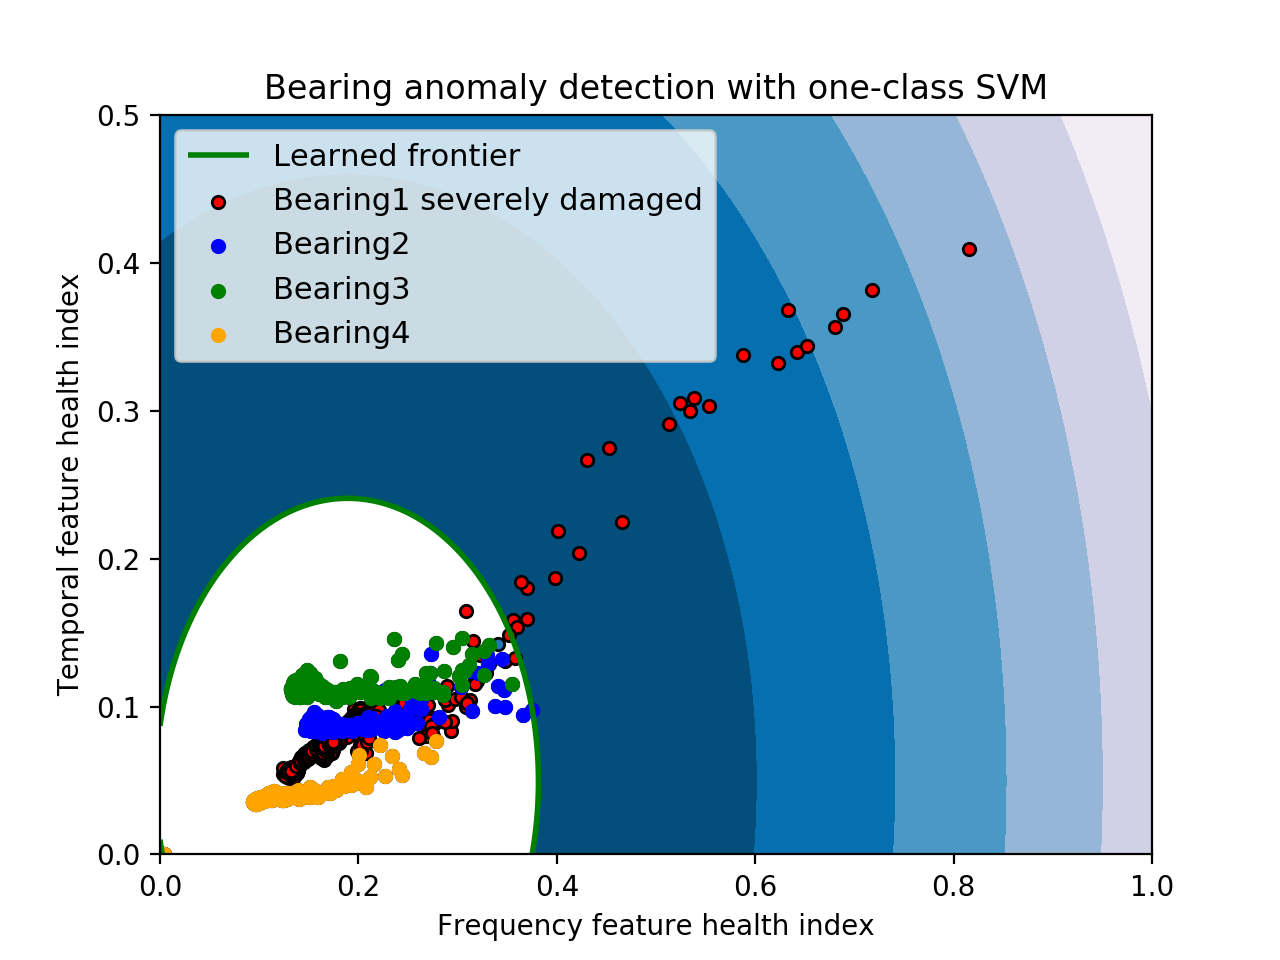
\includegraphics[width=0.5\linewidth]{svm}
		%\caption{}
		%\label{fig:datascience}
	\end{figure}
\end{frame}

%%%%%%%%%%%%%%%%%%%%%%%%%%%%%%%%%%%%%%%%%%%%%%%
\begin{frame}
		\frametitle{What else?}
			\begin{figure}[H]
			\centering
			
\includegraphics[width=0.7\linewidth]{question}
				\end{figure}
		
\end{frame}

\end{document}

